\documentclass[11pt,a4paper,twocolumn]{article}

\usepackage[T1]{fontenc}
\usepackage{lmodern}
\usepackage{microtype}
\usepackage[a4paper,top=16mm,bottom=16mm,left=16mm,right=16mm,columnsep=5.5mm,headheight=13pt]{geometry}
\usepackage{amsmath,amssymb}
\usepackage{booktabs,tabularx,array,multirow}
\usepackage{siunitx}
\usepackage[table]{xcolor}
\usepackage{graphicx}
\usepackage{tikz}
\usetikzlibrary{arrows.meta,positioning,fit,shapes.geometric,calc,matrix}
\usepackage{caption}
\usepackage{subcaption}
\usepackage{natbib}
\usepackage{fancyhdr}
\usepackage[hidelinks]{hyperref}
\usepackage[nameinlink,noabbrev]{cleveref}

\definecolor{ink}{HTML}{172A3A}
\definecolor{accent}{HTML}{176B87}
\definecolor{rulegray}{HTML}{A8B3BC}
\definecolor{rowblue}{HTML}{EEF5F7}
\definecolor{notegray}{HTML}{F3F5F6}
\definecolor{navy}{HTML}{16324F}
\definecolor{blue}{HTML}{2563A6}
\definecolor{cyan}{HTML}{2A9D8F}
\definecolor{gold}{HTML}{E9A23B}
\definecolor{red}{HTML}{C84C4C}
\definecolor{lightblue}{HTML}{EAF2F8}
\definecolor{lightgray}{HTML}{F3F5F7}
\definecolor{darkgray}{HTML}{4B5563}
\definecolor{openaiC}{HTML}{2F5597}
\definecolor{anthropicC}{HTML}{C44E52}
\definecolor{googleC}{HTML}{E69F00}
\definecolor{deepseekC}{HTML}{009E73}
\definecolor{xaiC}{HTML}{7F3C8D}

\hypersetup{
  pdftitle={Beyond Correctness: A Controlled Benchmark of AI Models on Advanced University Mathematics and Physics},
  pdfauthor={Francesco Bortot},
  pdfsubject={Closed-resource benchmark of mathematical and physical problem solving},
  pdfkeywords={large language models, mathematical reasoning, physics, benchmark, rubric evaluation, cost, latency},
  colorlinks=true,
  linkcolor=ink,
  citecolor=accent,
  urlcolor=accent
}

\pagestyle{fancy}
\fancyhf{}
\fancyhead[L]{\footnotesize Beyond correctness in university problem solving}
\fancyhead[R]{\footnotesize Bortot}
\fancyfoot[C]{\footnotesize\thepage}
\renewcommand{\headrulewidth}{0.3pt}
\renewcommand{\footrulewidth}{0pt}

\setlength{\parindent}{1em}
\setlength{\parskip}{0pt}
\setlength{\emergencystretch}{1.5em}
\setlength{\textfloatsep}{8pt plus 2pt minus 2pt}
\setlength{\floatsep}{7pt plus 2pt minus 2pt}
\setlength{\intextsep}{7pt plus 2pt minus 2pt}
\renewcommand{\topfraction}{0.95}
\renewcommand{\bottomfraction}{0.90}
\renewcommand{\textfraction}{0.04}
\renewcommand{\floatpagefraction}{0.86}
\renewcommand{\dbltopfraction}{0.96}
\renewcommand{\dblfloatpagefraction}{0.86}
\setcounter{dbltopnumber}{3}
\makeatletter
\setlength{\@dblfptop}{0pt}
\setlength{\@dblfpsep}{10pt}
\setlength{\@dblfpbot}{0pt plus 1fil}
\makeatother
\captionsetup{font=footnotesize,labelfont=bf,labelsep=period}
\sisetup{detect-all,group-separator={,},group-minimum-digits=4}

\newcommand{\snapshotdate}{14 August 2026}
\newcommand{\code}[1]{\texttt{\detokenize{#1}}}
\newcommand{\repo}[1]{\nolinkurl{#1}}
\newcolumntype{Y}{>{\raggedright\arraybackslash}X}
\newcolumntype{C}{>{\centering\arraybackslash}X}
\newcolumntype{P}[1]{>{\raggedright\arraybackslash}p{#1}}

\begin{document}
\raggedbottom

\twocolumn[
\begin{@twocolumnfalse}
\begin{center}
  {\LARGE\bfseries Beyond Correctness:\par}
  \vspace{0.12em}
  {\Large\bfseries A Controlled Benchmark of AI Models on Advanced University Mathematics and Physics\par}
  \vspace{0.7em}
  {\large Francesco Bortot\par}
  \vspace{0.22em}
  {\small Benchmark and analysis snapshot: \snapshotdate\par}
\end{center}

\vspace{0.3em}
\noindent\rule{\textwidth}{0.6pt}
\vspace{0.5em}

\begin{minipage}{0.96\textwidth}
\small
\textbf{Abstract.}
Open-ended university problems expose whether a model can construct and verify
a solution rather than merely recognize an answer. The objective is to compare
solution correctness and completeness together with the resources required to
obtain them. A controlled, closed-resource benchmark evaluates 14 model--mode
configurations on 60 authentic examination problems in Mathematical Analysis
III and General Physics II. Sixty item-specific rubrics contain 1,600 atomic
criteria; answers are assessed anonymously in
single-response contexts, centrally validated, and every case of substantive
doubt is escalated to versioned human adjudication. The six leading
configurations occupy a narrow 96.71--98.72\% band, and paired bootstrap
intervals do not separate the first system from its two nearest competitors.
In a same-weights DeepSeek V4 Flash contrast, high reasoning adds 10.93
percentage points (95\% CI 7.97--14.10), while increasing token use by 214.7\%,
cost by 224.4\%, and median latency 5.13-fold. Across the normalized matched
panel, model-level analytical-token volume, estimated API cost, and median
latency vary by factors of 6.91, 234.61, and 12.46. These results show
that, once correctness approaches saturation, resource demand, robustness
across domains, and quality--resource frontiers become central outcomes.

\vspace{0.4em}
\noindent\textbf{Keywords:} large language models; mathematical reasoning;
physics problem solving; blind rubric evaluation; efficiency; latency.
\end{minipage}
\vspace{0.65em}
\end{@twocolumnfalse}
]

\section{Introduction}

Scientific problem solving is an unusually demanding test of language models.
An acceptable response must identify the mathematical or physical structure,
select a defensible method, execute a multi-step derivation, respect domains or
units, and communicate a complete conclusion. Exact-match answers collapse
these requirements into one bit: they miss invalid derivations that happen to
end correctly and substantial correct work followed by a local error.

The same limitation now affects model ranking. When several systems solve most
items correctly, small differences in mean score may be weaker than their
sampling uncertainty, while latency, hidden reasoning, and price can differ by
orders of magnitude. A benchmark intended for model selection must therefore
measure not only whether a solution is correct but also how it is correct and
what is consumed to produce it.

This study addresses three questions. \emph{RQ1} asks how accurately and
completely 14 current configurations solve the same 60 advanced examination
problems, including the residual criterion-level structure behind their
scores. \emph{RQ2} asks whether performance is stable between Mathematical
Analysis III and General Physics II. \emph{RQ3} asks how quality relates to
token volume, dated estimated API cost, and end-to-end response time. One
same-weights thinking/no-thinking pair additionally provides a focused
configuration contrast.

The contribution is a traceable measurement architecture rather than a larger
question bank. Authentic examination material is combined with a direct-API,
one-item, no-tool execution condition; frozen item-specific atomic rubrics;
blind single-answer assessment; permanent response-to-identity mappings;
central validation; and human authority resolution before unblinding. The
result is a balanced 14-by-60 panel in which correctness and resource
measurements refer to exactly the same model--item cells.

\section{Related Work and Positioning}\label{sec:related-work}

Scientific benchmarks span broad college-level problem solving, expert-written
graduate questions, undergraduate physics coverage, open-answer validation,
and step-level reasoning. SciBench and GPQA established complementary breadth
and expert difficulty; UGPhysics broadened undergraduate physics and hybrid
grading; PHYSICS and PhysReason emphasized open derivations and intermediate
reasoning \citep{wang2024scibench,rein2024gpqa,xu2025ugphysics,
feng2025physics,zhang2025physreason}. More recent benchmarks emphasize original
problem construction or multimodal decompositions of variables, processes,
and solutions \citep{qiu2025phybench,dai2025physicsarena}. The present study is
smaller by design: its unit is an authentic examination exercise evaluated in
depth against a frozen, inspectable scoring contract.

Benchmark governance is equally important. HELM motivates standardized
conditions and multidimensional reporting; BetterBench emphasizes lifecycle
documentation and reproducibility; contamination studies and LiveBench caution
against treating static scores as timeless evidence
\citep{liang2023helm,reuel2024betterbench,deng2024contamination,
white2025livebench}. Here, exact prompts, configurations, raw outputs, judgments,
adjudications, exclusions, and dated resource prices are part of the measured
artifact chain.

Model-based evaluation makes criterion-level grading scalable, but it can
introduce position, verbosity, self-preference, and self-recognition biases
\citep{zheng2023judge,hashemi2024llmrubric,
panickssery2024self,verga2024juries}. Model judgments are therefore treated as
provisional measurements rather than final authority. Solver identities and
competing responses are hidden, rubrics are fixed before scoring, every
judgment must cite evidence and pass deterministic validation, and substantive
uncertainty is escalated to human adjudication. Reliance on a single judge
family nevertheless remains a limitation.

\Cref{tab:benchmark-positioning} positions the present protocol through
documented design choices rather than binary feature claims or an implied
ranking of benchmark quality.

\begin{table*}[!t]
\centering
\caption{Protocol-level positioning against representative scientific-reasoning
benchmarks cited above. Entries summarize documented task and evaluation
designs; they do not rank overall benchmark quality.}
\label{tab:benchmark-positioning}
\footnotesize
\setlength{\tabcolsep}{3.2pt}
\renewcommand{\arraystretch}{1.08}
\begin{tabularx}{\textwidth}{P{2.75cm}P{4.0cm}P{5.0cm}Y}
\toprule
\textbf{Benchmark} & \textbf{Task and source} & \textbf{Response and scoring design} &
\textbf{Human and operational scope} \\
\midrule
SciBench \citep{wang2024scibench} & College mathematics, chemistry, and
physics; textbooks plus a smaller course-exam subset & Open solutions with
primarily final-answer assessment & Broad collegiate coverage and manual error
analysis \\
GPQA \citep{rein2024gpqa} & Expert-authored graduate biology, chemistry, and
physics questions & Four-option multiple choice with exact-choice accuracy &
Expert item validation and revision \\
UGPhysics \citep{xu2025ugphysics} & Undergraduate physics exercise books
covering multiple subjects & Open solutions and seven answer types; rule- and
model-based grading & Human validation of evaluator samples and token analyses \\
PHYSICS \citep{feng2025physics} & Public physics qualifying examinations &
Open solutions; regular-expression or symbolic checks with model fallback &
Expert annotation and cross-checking \\
PhysReason \citep{zhang2025physreason} & Entrance, practice, and competition
physics problems & Answer- and step-level scoring of open reasoning & Human
validation of evaluator outputs \\
\rowcolor{rowblue}
\textbf{This work} & 60 items from 20 dated university course examinations &
Open derivations; frozen atomic rubrics and blind single-answer judging &
Case-level human adjudication and paired token, cost, and latency measurements \\
\bottomrule
\end{tabularx}
\end{table*}

No individual element in the final row is claimed as unique. The contribution
is their integration within one auditable authority chain: authentic dated
examinations, frozen atomic rubrics, blind judgments, mandatory human resolution
of substantive doubt, and resource measurements all refer to the same cells.

\begin{figure*}[!t]
\centering
\resizebox{0.96\textwidth}{!}{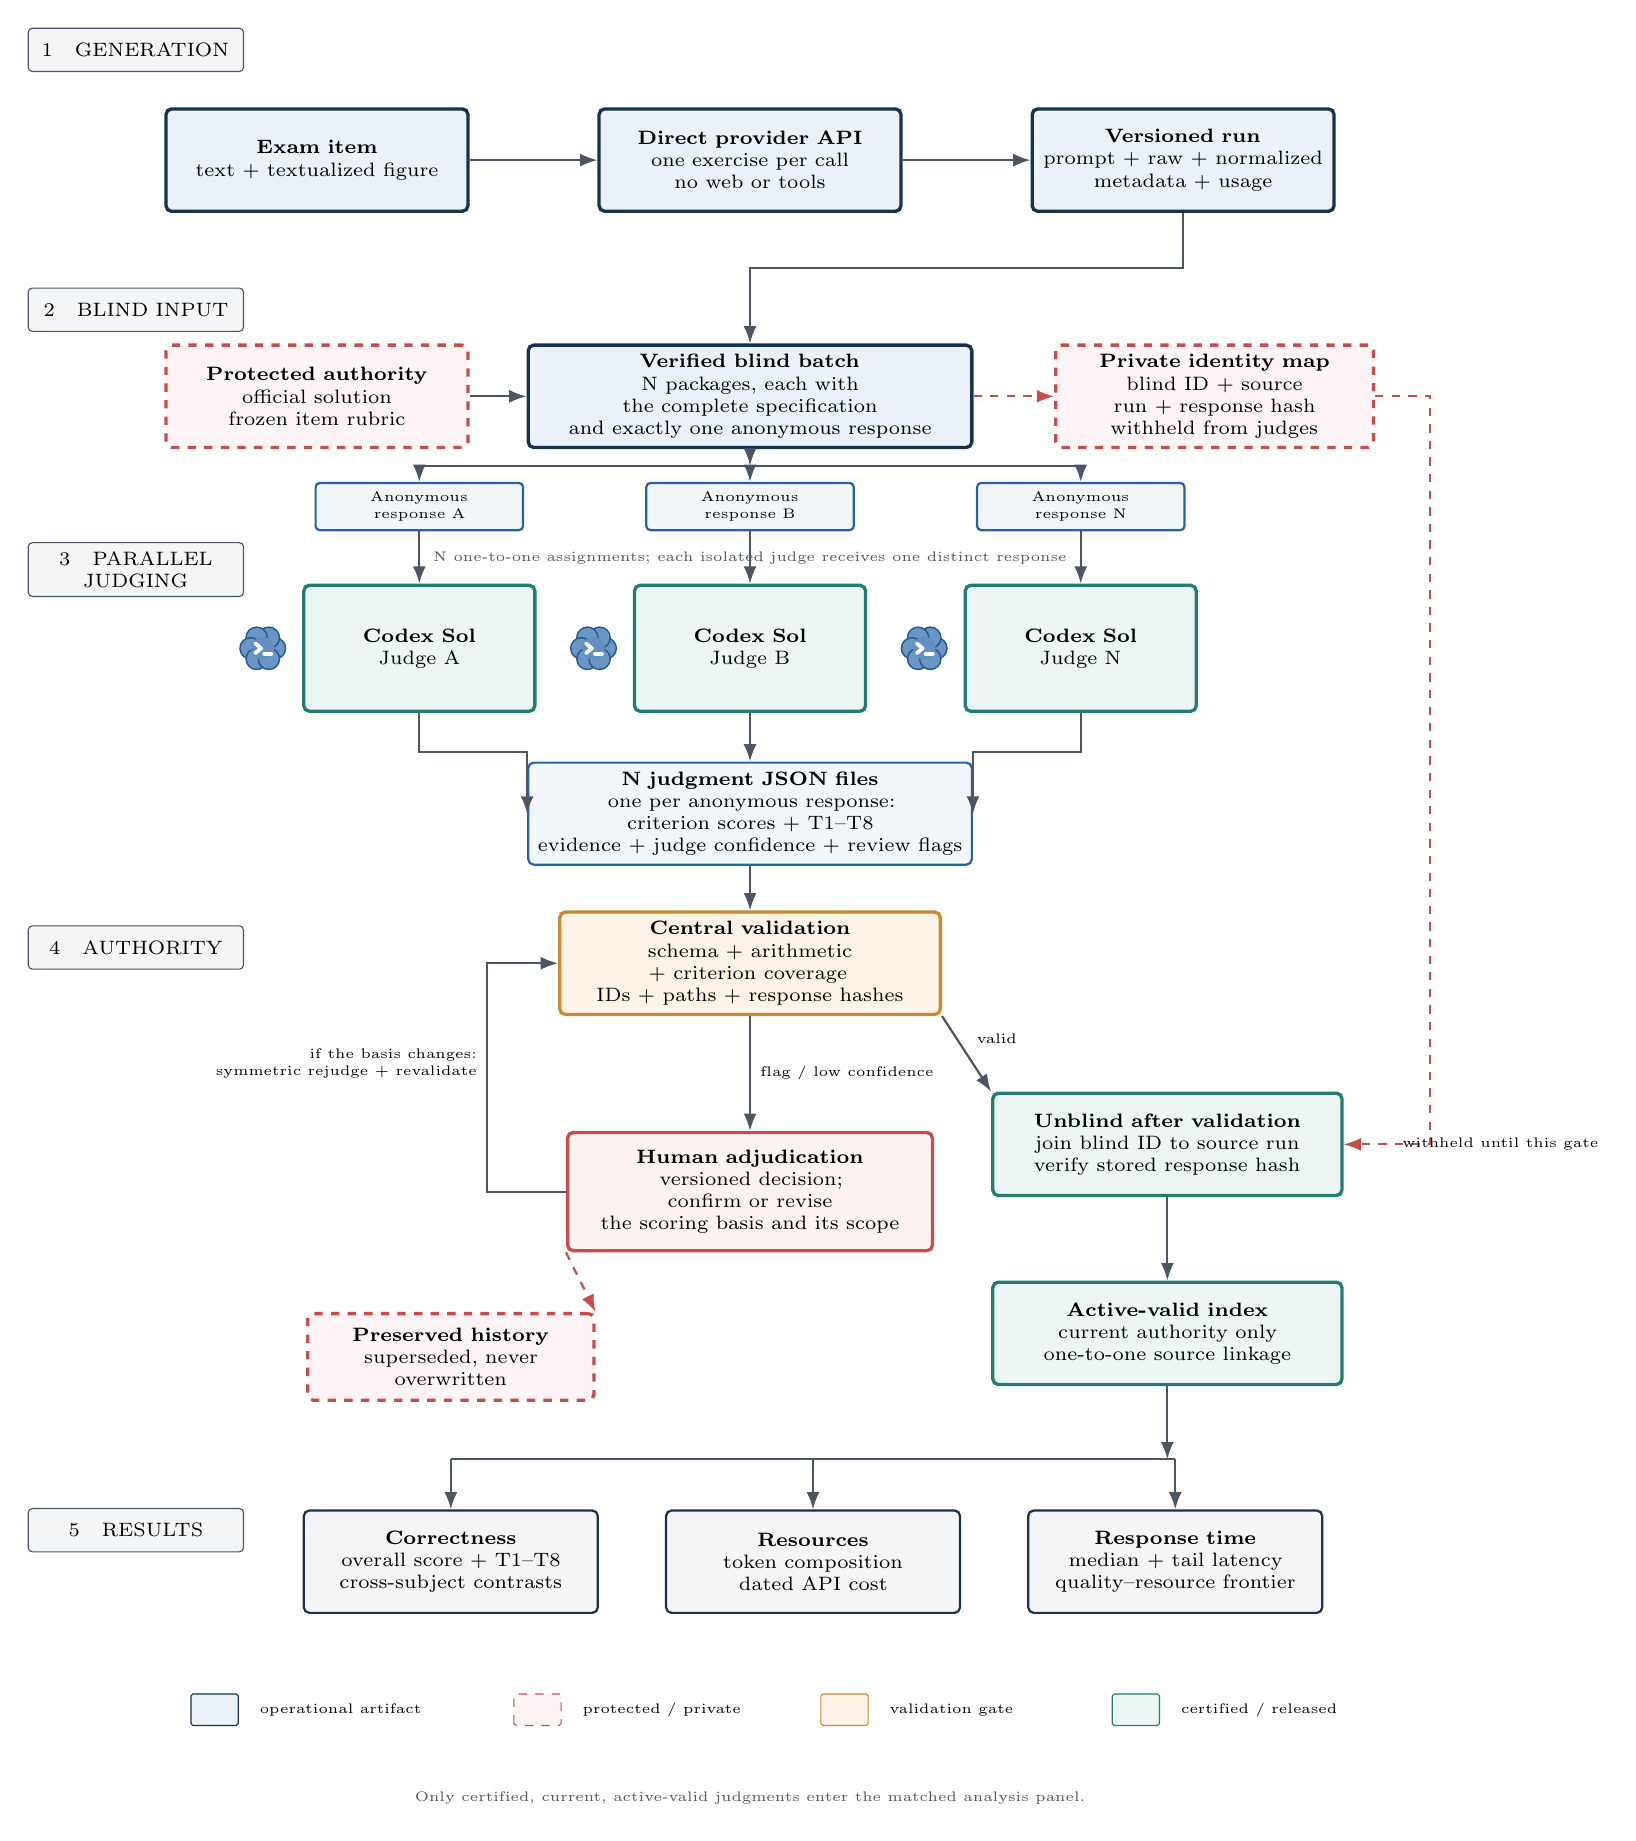
\begin{tikzpicture}[x=1mm,y=1mm,
  font=\scriptsize,
  main/.style={
    rounded corners=2pt,
    draw=navy,
    very thick,
    fill=lightblue,
    align=center,
    minimum height=13mm,
    text width=36mm
  },
  protected/.style={
    rounded corners=2pt,
    draw=red,
    very thick,
    dashed,
    fill=red!6,
    align=center,
    minimum height=13mm,
    text width=36mm
  },
  agent/.style={
    rounded corners=2pt,
    draw=cyan!80!black,
    very thick,
    fill=cyan!9,
    align=center,
    minimum height=16mm,
    text width=27mm
  },
  assignment/.style={
    rounded corners=1.5pt,
    draw=blue,
    thick,
    fill=blue!6,
    align=center,
    minimum height=6mm,
    text width=24mm,
    font=\tiny
  },
  artifact/.style={
    rounded corners=2pt,
    draw=blue,
    thick,
    fill=blue!6,
    align=center,
    minimum height=11mm,
    text width=54mm
  },
  validate/.style={
    rounded corners=2pt,
    draw=gold!85!black,
    very thick,
    fill=gold!13,
    align=center,
    minimum height=13mm,
    text width=46mm
  },
  human/.style={
    rounded corners=2pt,
    draw=red,
    very thick,
    fill=red!7,
    align=center,
    minimum height=15mm,
    text width=44mm
  },
  release/.style={
    rounded corners=2pt,
    draw=cyan!80!black,
    very thick,
    fill=cyan!9,
    align=center,
    minimum height=13mm,
    text width=39mm
  },
  result/.style={
    rounded corners=2pt,
    draw=navy,
    thick,
    fill=navy!5,
    align=center,
    minimum height=13mm,
    text width=35mm
  },
  phase/.style={
    rounded corners=1.5pt,
    draw=darkgray,
    fill=lightgray,
    font=\scriptsize,
    align=center,
    minimum height=5.5mm,
    text width=25mm
  },
  arrow/.style={-{Latex[length=2.2mm]},thick,draw=darkgray},
  protectedarrow/.style={-{Latex[length=2.2mm]},thick,dashed,draw=red},
  bus/.style={thick,draw=darkgray},
  pics/codexmark/.style={code={
    \foreach \ang in {0,60,...,300}{
      \filldraw[fill=blue!68,draw=blue!90!black,line width=0.18mm]
        (\ang:1.55mm) circle (1.35mm);
    }
    \fill[blue!72] (0,0) circle (1.45mm);
    \draw[white,line width=0.48mm,line cap=round,line join=round]
      (-0.95mm,0.62mm) -- (-0.20mm,0) -- (-0.95mm,-0.62mm);
    \draw[white,line width=0.48mm,line cap=round]
      (0.18mm,-0.68mm) -- (1.08mm,-0.68mm);
  }}
]
  % Phase 1: solver generation and durable run artifacts.
  \node[phase] at (-78,96) {1\quad GENERATION};
  \node[main] (item) at (-55,82)
    {\textbf{Exam item}\\text + textualized figure};
  \node[main] (api) at (0,82)
    {\textbf{Direct provider API}\\one exercise per call\\no web or tools};
  \node[main] (run) at (55,82)
    {\textbf{Versioned run}\\prompt + raw + normalized\\metadata + usage};
  \draw[arrow] (item) -- (api);
  \draw[arrow] (api) -- (run);

  % Phase 2: blind preparation and parallel Codex judges.
  \node[phase] at (-78,63) {2\quad BLIND INPUT};
  \node[protected] (reference) at (-55,52)
    {\textbf{Protected authority}\\official solution\\frozen item rubric};
  \node[main,text width=54mm] (blind) at (0,52)
    {\textbf{Verified blind batch}\\N packages, each with the complete specification\\and exactly one anonymous response};
  \node[protected,text width=38mm] (map) at (59,52)
    {\textbf{Private identity map}\\blind ID + source run + response hash\\withheld from judges};
  \draw[arrow] (reference) -- (blind);
  \draw[arrow] (run.south) -- ++(0,-7mm) -| (blind.north);
  \draw[protectedarrow] (blind) -- (map);

  \node[phase] at (-78,30) {3\quad PARALLEL JUDGING};
  \node[assignment] (responseA) at (-42,38)
    {Anonymous response A};
  \node[assignment] (responseB) at (0,38)
    {Anonymous response B};
  \node[assignment] (responseN) at (42,38)
    {Anonymous response N};
  \node[font=\tiny,text=darkgray,align=center] at (0,31.5)
    {N one-to-one assignments; each isolated judge receives one distinct response};
  \node[agent] (agentA) at (-42,20)
    {\textbf{Codex Sol}\\Judge A};
  \node[agent] (agentB) at (0,20)
    {\textbf{Codex Sol}\\Judge B};
  \node[agent] (agentN) at (42,20)
    {\textbf{Codex Sol}\\Judge N};
  \pic at ([xshift=-5mm]agentA.west) {codexmark};
  \pic at ([xshift=-5mm]agentB.west) {codexmark};
  \pic at ([xshift=-5mm]agentN.west) {codexmark};

  \coordinate (dispatch) at (0,43.2);
  \draw[arrow] (blind.south) -- (dispatch);
  \draw[bus] (-42,43.2) -- (42,43.2);
  \draw[arrow] (-42,43.2) -- (responseA.north);
  \draw[arrow] (0,43.2) -- (responseB.north);
  \draw[arrow] (42,43.2) -- (responseN.north);
  \draw[arrow] (responseA.south) -- (agentA.north);
  \draw[arrow] (responseB.south) -- (agentB.north);
  \draw[arrow] (responseN.south) -- (agentN.north);

  \node[artifact] (json) at (0,-1)
    {\textbf{N judgment JSON files}\\one per anonymous response: criterion scores + T1--T8\\evidence + judge confidence + review flags};
  \draw[arrow] (agentA.south) -- ++(0,-5mm) -| (json.west);
  \draw[arrow] (agentB) -- (json);
  \draw[arrow] (agentN.south) -- ++(0,-5mm) -| (json.east);

  % Phase 4: validation, adjudication, unblinding, and analysis.
  \node[phase] at (-78,-18) {4\quad AUTHORITY};
  \node[validate] (validator) at (0,-20)
    {\textbf{Central validation}\\schema + arithmetic + criterion coverage\\IDs + paths + response hashes};
  \draw[arrow] (json) -- (validator);

  \node[human] (human) at (0,-49)
    {\textbf{Human adjudication}\\versioned decision; confirm or revise\\the scoring basis and its scope};
  \node[release,text width=42mm] (unblind) at (53,-43)
    {\textbf{Unblind after validation}\\join blind ID to source run\\verify stored response hash};
  \draw[arrow] (validator.south) -- node[right,font=\tiny] {flag / low confidence} (human.north);
  \draw[arrow] (validator.south east) -- node[above right,font=\tiny] {valid} (unblind.north west);
  \draw[arrow] (human.west) -- ++(-10mm,0) |- node[pos=0.28,left,font=\tiny,align=right] {if the basis changes:\\symmetric rejudge + revalidate} (validator.west);
  \draw[protectedarrow] (map.east) -- ++(7mm,0) |- node[pos=0.72,right,font=\tiny] {withheld until this gate} (unblind.east);

  \node[protected,text width=34mm,minimum height=11mm] (history) at (-38,-70)
    {\textbf{Preserved history}\\superseded, never overwritten};
  \node[release,text width=42mm] (index) at (53,-67)
    {\textbf{Active-valid index}\\current authority only\\one-to-one source linkage};
  \draw[protectedarrow] (human.south west) -- (history.north east);
  \draw[arrow] (unblind) -- (index);

  \node[phase] at (-78,-92) {5\quad RESULTS};
  \node[result] (correct) at (-38,-96)
    {\textbf{Correctness}\\overall score + T1--T8\\cross-subject contrasts};
  \node[result] (resources) at (8,-96)
    {\textbf{Resources}\\token composition\\dated API cost};
  \node[result] (latency) at (54,-96)
    {\textbf{Response time}\\median + tail latency\\quality--resource frontier};
  \coordinate (resultbus) at (53,-83);
  \draw[arrow] (index.south) -- (resultbus);
  \draw[bus] (-38,-83) -- (54,-83);
  \draw[arrow] (-38,-83) -- (correct.north);
  \draw[arrow] (8,-83) -- (resources.north);
  \draw[arrow] (54,-83) -- (latency.north);

  \draw[draw=navy,fill=lightblue,rounded corners=0.7pt] (-71,-116.8) rectangle (-65,-112.8);
  \node[font=\tiny,anchor=west] at (-63.5,-114.8) {operational artifact};
  \draw[draw=red,dashed,fill=red!6,rounded corners=0.7pt] (-30,-116.8) rectangle (-24,-112.8);
  \node[font=\tiny,anchor=west] at (-22.5,-114.8) {protected / private};
  \draw[draw=gold!85!black,fill=gold!13,rounded corners=0.7pt] (9,-116.8) rectangle (15,-112.8);
  \node[font=\tiny,anchor=west] at (16.5,-114.8) {validation gate};
  \draw[draw=cyan!80!black,fill=cyan!9,rounded corners=0.7pt] (46,-116.8) rectangle (52,-112.8);
  \node[font=\tiny,anchor=west] at (53.5,-114.8) {certified / released};

  \node[font=\tiny,text=darkgray,align=center] at (0,-126)
    {Only certified, current, active-valid judgments enter the matched analysis panel.};
\end{tikzpicture}
}
\caption{Benchmark architecture and authority chain. The judging lanes denote
distinct anonymous responses: a batch of N responses produces N
one-to-one assignments, each handled in an isolated context, rather than three
judgments of the same answer. Generation is separated from evaluation, central
validation gates unblinding, and human review resolves substantive doubt. Only
a change to the common scoring basis triggers symmetric rejudging of all
affected answers. The three result branches correspond to the analyses in
\cref{sec:results}.}
\label{fig:architecture}
\end{figure*}

\section{Benchmark Design}

\subsection{Corpus and task condition}

The corpus contains 20 examination papers from the 2025 and 2026 sessions of
two advanced courses in a physics degree. Each paper contributes exactly three
open-ended exercises. The balanced population contains 33 Analysis III items
and 27 Physics II items. Analysis problems cover differential manifolds,
geometry, and differential equations; Physics II covers electromagnetism,
circuits, waves, and geometrical optics. Every item is linked to its official
solution and an approved operational rubric.

Original examination PDFs are retained as provenance records, while statements
and official solutions are transcribed to UTF-8 without silent correction.
Any disagreement among the scan, transcription, official solution, and rubric
enters human review. Essential figures were replaced by one authorized textual
description used unchanged for generation, rubric construction, and judgment. The resulting
track measures reasoning from controlled text, not visual perception. Each
solver received one exercise per call and a fixed response contract requiring
assumptions, method, verifiable development, separated final results, and
relevant checks. Web access, retrieval, code execution, calculators, and all
other tools were prohibited both in the prompt and in the API configuration.

\begin{center}
\begin{minipage}{\columnwidth}
\centering
\captionof{table}{Certified analysis population. Responses include repeated calls;
model--item cells are the macro-averaged unit used in comparisons.}
\label{tab:population}
\footnotesize
\setlength{\tabcolsep}{3.1pt}
\renewcommand{\arraystretch}{1.04}
\begin{tabularx}{\columnwidth}{Y r}
\toprule
\textbf{Component} & \textbf{Count} \\
\midrule
Examination papers / exercises & 20 / 60 \\
Analysis III / Physics II items & 33 / 27 \\
Model--mode configurations & 14 \\
Active responses, including replications & 924 \\
Balanced model--item cells & 840 \\
Frozen rubrics / rubric subproblems & 60 / 214 \\
Atomic scoring criteria & 1,600 \\
Open human-review cases at snapshot & 0 \\
\bottomrule
\end{tabularx}
\end{minipage}
\end{center}

\subsection{Configurations and direct-API execution}

All generation requests were sent by the benchmark harness directly to the
first-party API of the selected provider. No aggregator, including OpenRouter,
was used. A versioned configuration fixed the model identifier, reasoning
mode, item set, prompt, repetition policy, concurrency, timeout, retry policy,
output ceiling, and dated price table. The effective prompt, normalized answer,
raw provider object, and technical metadata were persisted separately. Thus,
what the model saw, what the judge saw, and what the provider returned remain
independently reconstructible.

\Cref{tab:models} reports the exact identities in the balanced panel. Active
response counts exceed 60 for configurations that participated in early
campaign waves with three calls on selected 2025 items to observe within-cell
stochastic repeatability. Later completion waves used one call per missing cell
to extend matched coverage within the available budget. This wave-level design
choice was independent of answer quality, and replications are never treated as
new items.

\begin{table*}[!t]
\centering
\caption{Exact model--mode configurations. ``Active responses'' includes
replications before within-cell macro-averaging. API identifiers and
campaign-level modes are reported as configured.}
\label{tab:models}
\scriptsize
\setlength{\tabcolsep}{3.5pt}
\renewcommand{\arraystretch}{1.04}
\begin{tabularx}{\textwidth}{P{1.45cm}P{3.35cm}P{4.55cm}Y r}
\toprule
\textbf{Provider} & \textbf{Display name} & \textbf{Exact API identifier} &
\textbf{Configured mode} & \textbf{Active responses} \\
\midrule
OpenAI & GPT-5.6 Sol & \repo{gpt-5.6-sol} & reasoning, xhigh & 78 \\
OpenAI & o3 & \repo{o3-2025-04-16} & reasoning, high & 60 \\
OpenAI & GPT-4.1 & \repo{gpt-4.1-2025-04-14} & no native reasoning & 60 \\
\addlinespace[1pt]
Anthropic & Claude Fable 5 & \repo{claude-fable-5} & effort, high & 78 \\
Anthropic & Claude Sonnet 4.5 & \repo{claude-sonnet-4-5-20250929} & provider default & 60 \\
Anthropic & Claude Haiku 4.5 & \repo{claude-haiku-4-5-20251001} & no thinking parameter requested & 60 \\
\addlinespace[1pt]
Google & Gemini 3.1 Pro Preview & \repo{gemini-3.1-pro-preview} & native reasoning & 78 \\
Google & Gemini 3.5 Flash & \repo{gemini-3.5-flash} & thinking, high & 90 \\
Google & Gemma 4 31B IT & \repo{gemma-4-31b-it} & thinking disabled & 60 \\
\addlinespace[1pt]
DeepSeek & V4 Flash & \repo{deepseek-v4-flash} & thinking enabled, reasoning high & 60 \\
DeepSeek & V4 Flash (no thinking) & \repo{deepseek-v4-flash} & thinking disabled & 60 \\
DeepSeek & V4 Pro & \repo{deepseek-v4-pro} & thinking enabled, reasoning high & 60 \\
\addlinespace[1pt]
xAI & Grok 4.5 & \repo{grok-4.5} & reasoning, high & 60 \\
xAI & Grok 4.3 & \repo{grok-4.3} & reasoning, high & 60 \\
\bottomrule
\end{tabularx}
\end{table*}

\subsection{Run provenance and resource boundaries}

Metadata record timestamps, attempts, finish reason, latency, provider token
fields, cost provenance, and prompt and response hashes. Resume and retry never
overwrite a completed historical artifact. The repository-wide index contains
977 run records.\footnote{Six are failed unavailable-endpoint calls, and 47
are completed Gemini 3.1 Flash-Lite runs excluded because that configuration
does not cover the complete 60-item panel. Among the 924 retained responses,
798 model--item cells have one run and 42 have three: nine cells each for
GPT-5.6 Sol, Claude Fable 5, and Gemini 3.1 Pro Preview, and 15 for Gemini 3.5
Flash. The 84 additional runs are averaged within their cells.}
The balanced analysis therefore retains 924 successful responses belonging to
the 14 configurations in \cref{tab:models}, then reduces them to 840 equally
weighted model--item cells before between-model comparison.

Analytical tokens are input plus visible output plus separately reported
reasoning. For Claude Fable 5, the provider exposes a combined output/thinking
quantity, which is retained as an unseparated class. Costs are provider-reported
for 120 of the 840 cells and reconstructed from versioned campaign rates for
720. Resource totals used for between-model comparison are computed after
within-cell macro-averaging and therefore describe an equal-weight 840-cell
panel, not billed campaign expenditure. Before averaging, the 924 retained
successful responses correspond to 10,054,390 analytical tokens and an
estimated \$105.10 under the same hybrid accounting; this still excludes
unobserved failed attempts and calls outside the matched panel. At least one
request required retry in 22 cells. Token and cost fields record the final
successful generation only, because consumption from failed attempts is not
available. Latency is measured from the first dispatch to the successful
return, so it includes provider processing, backoff, and retry delays but not
time spent waiting for a local concurrency slot.

\section{Blind Evaluation and Analysis}

\subsection{Frozen atomic rubrics}

Rubrics were constructed from the item, official solution, and authorized
figure description before model answers were examined. The 60 rubrics contain
214 weighted subproblems and 1,600 atomic criteria: 837 criteria for the 33
Analysis III items and 763 for the 27 Physics II items. Each criterion specifies
full-credit evidence, four partial-credit anchors, zero conditions, accepted
equivalences, alternative methods, and propagated-error policy. Physics
criteria additionally encode tolerances, units, directions, phases, and
peak/RMS conventions. Style and verbosity receive no points.

\begin{figure*}[!t]
\centering
\resizebox{0.96\textwidth}{!}{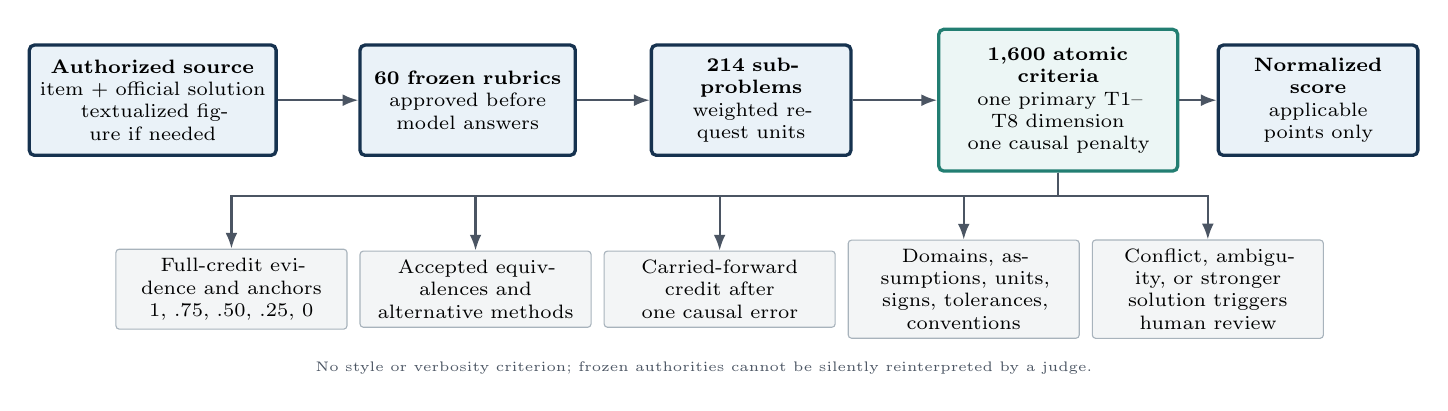
\begin{tikzpicture}[x=1mm,y=1mm,font=\scriptsize,
  box/.style={rounded corners=1.8pt,draw=navy,very thick,fill=lightblue,
    align=center,minimum height=14mm},
  atom/.style={rounded corners=1.8pt,draw=cyan!80!black,very thick,fill=cyan!9,
    align=center,minimum height=18mm},
  detail/.style={rounded corners=1.2pt,draw=rulegray,fill=notegray,
    align=center,minimum height=8mm,text width=27mm},
  arr/.style={-{Latex[length=2mm]},thick,draw=darkgray}]

  \node[box,text width=29mm] (source) at (-70,16)
    {\textbf{Authorized source}\\item + official solution\\textualized figure if needed};
  \node[box,text width=25mm] (rubric) at (-30,16)
    {\textbf{60 frozen rubrics}\\approved before model answers};
  \node[box,text width=23mm] (sub) at (6,16)
    {\textbf{214 subproblems}\\weighted request units};
  \node[atom,text width=28mm] (criteria) at (45,16)
    {\textbf{1,600 atomic criteria}\\one primary T1--T8 dimension\\one causal penalty};
  \node[box,text width=23mm] (score) at (78,16)
    {\textbf{Normalized score}\\applicable points only};
  \draw[arr] (source) -- (rubric);
  \draw[arr] (rubric) -- (sub);
  \draw[arr] (sub) -- (criteria);
  \draw[arr] (criteria) -- (score);

  \node[detail] (evidence) at (-60,-8)
    {Full-credit evidence and anchors\\{1, .75, .50, .25, 0}};
  \node[detail] (equiv) at (-29,-8)
    {Accepted equivalences and\\alternative methods};
  \node[detail] (prop) at (2,-8)
    {Carried-forward credit after\\one causal error};
  \node[detail] (phys) at (33,-8)
    {Domains, assumptions, units,\\signs, tolerances, conventions};
  \node[detail] (review) at (64,-8)
    {Conflict, ambiguity, or stronger\\solution triggers human review};
  \draw[arr] (criteria.south) -- ++(0,-3mm) -| (evidence.north);
  \draw[arr] (criteria.south) -- ++(0,-3mm) -| (equiv.north);
  \draw[arr] (criteria.south) -- ++(0,-3mm) -| (prop.north);
  \draw[arr] (criteria.south) -- ++(0,-3mm) -| (phys.north);
  \draw[arr] (criteria.south) -- ++(0,-3mm) -| (review.north);

  \node[font=\tiny,text=darkgray,align=center] at (0,-18)
    {No style or verbosity criterion; frozen authorities cannot be silently reinterpreted by a judge.};
\end{tikzpicture}
}
\caption{Anatomy of the scoring contract. A criterion is answer-independent,
belongs to one primary technical dimension, and can penalize one causal error
only once. Judges may flag a reference or rubric conflict, but they cannot
silently reinterpret a frozen authority.}
\label{fig:rubric}
\end{figure*}

Criteria map to the eight dimensions in \cref{tab:dimensions}. The final item
score is the percentage of points applicable to that exercise. T8 is applicable
to 14 Analysis III items only; it is not defined for the remaining 19 Analysis
III items or any Physics II item. This conditional denominator is preserved in
all profiles rather than imputing zero.

\begin{table*}[!t]
\centering
\caption{Technical dimensions and nominal budgets. The same high-level
dimensions govern both subjects; criterion evidence remains item-specific.}
\label{tab:dimensions}
\footnotesize
\setlength{\tabcolsep}{3.6pt}
\renewcommand{\arraystretch}{1.05}
\begin{tabularx}{\textwidth}{c r Y c r Y c r Y c r Y}
\toprule
\textbf{Dim.} & \textbf{Pts} & \textbf{Construct} &
\textbf{Dim.} & \textbf{Pts} & \textbf{Construct} &
\textbf{Dim.} & \textbf{Pts} & \textbf{Construct} &
\textbf{Dim.} & \textbf{Pts} & \textbf{Construct} \\
\midrule
T1 & 20 & Understanding / model & T2 & 15 & Method selection &
T3 & 20 & Development & T4 & 15 & Results / coverage \\
T5 & 10 & Conditions / conventions & T6 & 8 & Coherence / plausibility &
T7 & 7 & Theorems / laws & T8 & 5 & Independent verification \\
\bottomrule
\end{tabularx}
\end{table*}

\subsection{Blind judging, validation, and human authority}

Each first-pass judge received one anonymous response together with the full
subject specification, item, official solution, and frozen rubric. It did not
receive solver identity, competing answers, prior scores, or the private map.
For a batch of N responses, the system created N isolated Codex Sol assignments:
each assignment scored one distinct response, cited evidence for every applicable
criterion, calculated T1--T8, and emitted one structured judgment.
Before dispatch, every blind ID was bound permanently to one source run and
response hash; bijective map and manifest checks preceded the first judgment.

Central validation then checked schema, criterion coverage, arithmetic,
dimension sums, identifiers, unique paths, allowed values, and frozen-input
hashes. Only validated judgments could be unblinded. Blind single-answer
assessment prevents position effects and direct cross-model comparison at the
judging stage, but a single model-family judge can still introduce systematic
bias; this remains a limitation rather than being assumed away.

Every case of substantive doubt was reviewed by the human benchmark lead
before unblinding; no flagged case was resolved by the model judge alone. The
reviewer can confirm the frozen basis, recognize an equivalent or stronger
method, correct a reference or rubric, or identify a judge error. Decisions are
versioned and historical files remain preserved. Crucially, confirmation of
the existing basis changes only the flagged judgment, whereas a material
change to that basis initiates symmetric blind reassessment of every affected
answer. At the analysis snapshot, all planned judgments validated and
unblinded, with no unresolved human-review flag.\footnote{In the 282-response
completion wave---the final batch used to fill missing cells in the 14-by-60
panel---21 responses were blindly rejudged on previously approved adjudicated
bases. Five received score-preserving overlays, meaning versioned annotations
that incorporated an approved decision without changing the numerical score;
three run-validity classifications were overruled, also without score changes.}

\begin{table*}[!t]
\centering
\caption{Main matched-panel results. Score intervals are 20,000-resample
item-bootstrap intervals. Tokens and estimated cost are normalized panel totals
for 60 macro-averaged cells; time is the median model--item response time. Shading
marks the six-model near-ceiling group.}
\label{tab:main-results}
\scriptsize
\setlength{\tabcolsep}{3.6pt}
\renewcommand{\arraystretch}{1.04}
\begin{tabularx}{\textwidth}{rY r@{\ }l r r r r r}
\toprule
\textbf{Rank} & \textbf{Configuration} & \multicolumn{2}{c}{\textbf{Overall score [95\% CI]}} &
\textbf{Analysis III} & \textbf{Physics II} & \textbf{Tokens (M)} &
\textbf{Est. cost (USD)} & \textbf{Median (s)} \\
\midrule
\rowcolor{cyan!5}1 & GPT-5.6 Sol & 98.72 & [97.04, 99.86] & 99.86 & 97.33 & 0.959 & 27.8053 & 307.0 \\
\rowcolor{cyan!5}2 & Claude Fable 5 & 97.99 & [96.15, 99.38] & 98.44 & 97.45 & 0.507 & 22.9185 & 83.5 \\
\rowcolor{cyan!5}3 & DeepSeek V4 Flash & 97.24 & [94.66, 99.16] & 97.10 & 97.41 & 1.396 & 0.3845 & 188.0 \\
\rowcolor{cyan!5}4 & Gemini 3.1 Pro Preview & 97.05 & [95.11, 98.60] & 96.63 & 97.56 & 0.690 & 7.8895 & 114.7 \\
\rowcolor{cyan!5}5 & Gemini 3.5 Flash & 96.95 & [95.10, 98.51] & 97.29 & 96.53 & 0.976 & 8.4965 & 61.2 \\
\rowcolor{cyan!5}6 & DeepSeek V4 Pro & 96.71 & [94.76, 98.31] & 96.57 & 96.89 & 1.066 & 0.9102 & 202.4 \\
7 & Grok 4.5 & 94.61 & [91.66, 97.08] & 95.59 & 93.42 & 0.576 & 3.2504 & 113.8 \\
8 & OpenAI o3 & 92.75 & [89.74, 95.33] & 90.49 & 95.52 & 0.644 & 4.9216 & 70.2 \\
9 & DeepSeek V4 Flash (no thinking) & 86.31 & [82.73, 89.68] & 84.73 & 88.24 & 0.443 & 0.1185 & 36.6 \\
10 & Gemma 4 31B IT & 85.58 & [81.52, 89.34] & 82.80 & 88.98 & 0.209 & 0.0000 (cfg.) & 74.8 \\
11 & Grok 4.3 & 85.24 & [79.77, 90.11] & 80.40 & 91.16 & 0.656 & 1.5744 & 73.7 \\
12 & OpenAI GPT-4.1 & 71.58 & [66.46, 76.53] & 64.02 & 80.82 & 0.311 & 2.2599 & 39.1 \\
13 & Claude Sonnet 4.5 & 70.91 & [65.31, 76.41] & 60.71 & 83.37 & 0.202 & 2.4706 & 37.4 \\
14 & Claude Haiku 4.5 & 64.77 & [59.57, 69.80] & 57.59 & 73.54 & 0.279 & 1.2084 & 24.6 \\
\bottomrule
\multicolumn{9}{l}{\scriptsize cfg. marks a campaign-configured zero, not a general market price.}
\end{tabularx}
\end{table*}

\subsection{Aggregation and uncertainty}

The exercise is the sampling unit. For each configuration, repeated responses
are first averaged within their model--item cell, producing one score for each
of the same 60 exercises. The reported model mean is the arithmetic mean of
those 60 cell scores, so a triplicated cell has the same weight as a cell with
one response and every configuration remains directly paired by item.

Uncertainty is estimated with 20,000 nonparametric bootstrap iterations using
seed 20260810. In each iteration, 60 exercise indices are sampled with
replacement from the common item set. For every configuration, the mean is
recomputed from the cell scores at those sampled indices; the 2.5th and 97.5th
percentiles form the marginal 95\% interval. For a paired model contrast, the
same resampled indices are applied to both configurations before their means
are subtracted, preserving item-level pairing in every iteration. These
intervals quantify sensitivity to sampling exercises from this benchmark; they
do not include uncertainty from future provider changes or from replacing the
judge model.

Replications and bootstrap resampling address different uncertainties: the 42
triplicated cells observe generation variability for selected model--item
pairs, whereas the bootstrap resamples the 60 exercise identities to estimate
item-sampling uncertainty without imputing run variability to single-run cells.

Resource totals and subject means are calculated on the same macro-averaged
cells. Pareto fronts maximize score while minimizing one resource at a time;
no composite efficiency index or subjective exchange rate is imposed.
Correlations use the 14 model aggregates and are reported as descriptive
associations only.

\section{Results}\label{sec:results}

\subsection{A near-ceiling leading group}

\Cref{tab:main-results} is the numerical backbone of the results: every row
summarizes the same 60 items and joins quality to resource demand. The first six
configurations occupy only 2.01 percentage points, from 96.71\% to 98.72\%.
Their marginal intervals overlap substantially. More directly, the paired
difference between GPT-5.6 Sol and Claude Fable 5 is 0.72 pp (95\% CI
$-0.56$ to 1.95), and the difference between GPT-5.6 Sol and DeepSeek V4 Flash
is 1.48 pp (95\% CI $-0.23$ to 3.73). The observed order should therefore not
be read as fourteen precisely separated performance levels. ``Top-six'' is an
empirical near-ceiling label based on close estimates and overlapping intervals,
not a formal equivalence class; no equivalence margin was prespecified.

Across all 840 cells, 41.67\% are perfect and 91.19\% score at least 60\%; the
macro-mean is 88.31\%. These aggregates describe the selected panel, not an
expected score for an arbitrary model or course.

\Cref{fig:item-difficulty} shows that saturation is not uniform.
Exercise means span 50.84--99.68\%; 30 of 60 remain below 90\% and nine below
80\%, seven of them in Analysis III. The corpus therefore combines a broad
high-scoring region with a smaller, substantively discriminating tail.

\begin{figure*}[!t]
\centering
\resizebox{0.97\textwidth}{!}{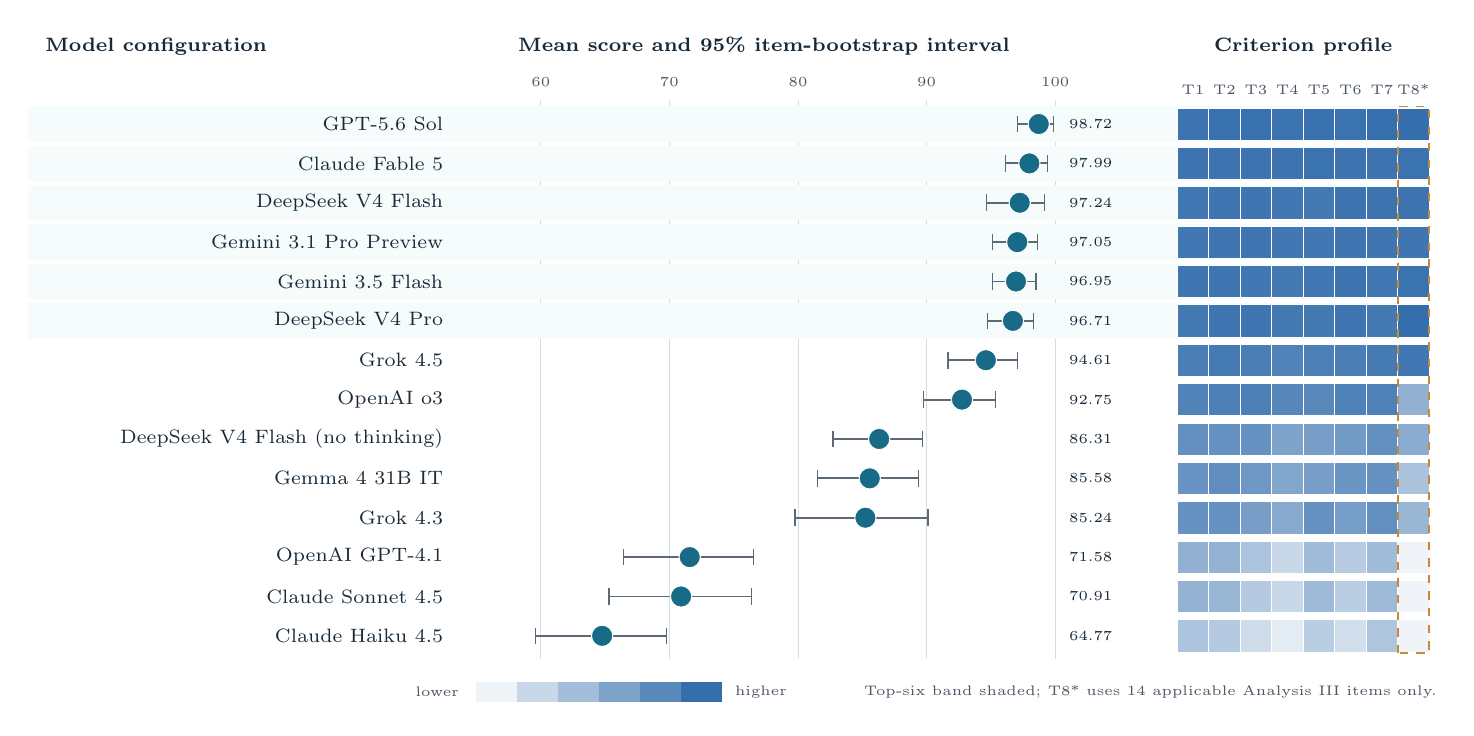
\begin{tikzpicture}[x=1mm,y=1mm,font=\scriptsize]
  \def\scoreleft{-31}
  \def\scorewidth{73.5}
  \def\heatleft{58}
  \def\cellw{4.00}
  \newcount\rankrowcount
  \rankrowcount=0

  % Column guides for the forest plot.
  \foreach \tick in {60,70,80,90,100}{
    \pgfmathsetmacro{\xtick}{\scoreleft+(\tick-55)*\scorewidth/45}
    \draw[rulegray!45,line width=0.25pt] (\xtick,3) -- (\xtick,-68);
    \node[font=\tiny,text=darkgray,anchor=south] at (\xtick,3.5) {\tick};
  }
  \node[font=\scriptsize\bfseries,anchor=south west,text=ink] at (-87,7.5)
    {Model configuration};
  \node[font=\scriptsize\bfseries,anchor=south,text=ink] at (5.5,7.5)
    {Mean score and 95\% item-bootstrap interval};
  \node[font=\scriptsize\bfseries,anchor=south,text=ink] at (74,7.5)
    {Criterion profile};

  \foreach \lab [count=\j from 0] in {T1,T2,T3,T4,T5,T6,T7,T8*}{
    \pgfmathsetmacro{\xh}{\heatleft+\j*\cellw+0.5*\cellw}
    \node[font=\tiny,text=darkgray] at (\xh,4.4) {\lab};
  }

  \newcommand{\rankrow}[4]{%
    \pgfmathsetmacro{\yy}{-5*\the\rankrowcount}
    \ifnum\rankrowcount<6
      \fill[cyan!4] (-88,\yy-2.25) rectangle (90,\yy+2.25);
    \fi
    \node[anchor=east,font=\scriptsize,text=ink] at (-34,\yy) {#1};
    \pgfmathsetmacro{\xm}{\scoreleft+(#2-55)*\scorewidth/45}
    \pgfmathsetmacro{\xl}{\scoreleft+(#3-55)*\scorewidth/45}
    \pgfmathsetmacro{\xh}{\scoreleft+(#4-55)*\scorewidth/45}
    \draw[ink!70,line width=0.65pt] (\xl,\yy) -- (\xh,\yy);
    \draw[ink!70,line width=0.45pt] (\xl,\yy-1.05) -- (\xl,\yy+1.05);
    \draw[ink!70,line width=0.45pt] (\xh,\yy-1.05) -- (\xh,\yy+1.05);
    \filldraw[fill=accent,draw=white,line width=0.35pt] (\xm,\yy) circle (1.35);
    \node[anchor=east,font=\tiny,text=ink] at (51,\yy) {#2};
    \advance\rankrowcount by 1
  }

  \rankrow{GPT-5.6 Sol}{98.72}{97.04}{99.86}
  \rankrow{Claude Fable 5}{97.99}{96.15}{99.38}
  \rankrow{DeepSeek V4 Flash}{97.24}{94.66}{99.16}
  \rankrow{Gemini 3.1 Pro Preview}{97.05}{95.11}{98.60}
  \rankrow{Gemini 3.5 Flash}{96.95}{95.10}{98.51}
  \rankrow{DeepSeek V4 Pro}{96.71}{94.76}{98.31}
  \rankrow{Grok 4.5}{94.61}{91.66}{97.08}
  \rankrow{OpenAI o3}{92.75}{89.74}{95.33}
  \rankrow{DeepSeek V4 Flash (no thinking)}{86.31}{82.73}{89.68}
  \rankrow{Gemma 4 31B IT}{85.58}{81.52}{89.34}
  \rankrow{Grok 4.3}{85.24}{79.77}{90.11}
  \rankrow{OpenAI GPT-4.1}{71.58}{66.46}{76.53}
  \rankrow{Claude Sonnet 4.5}{70.91}{65.31}{76.41}
  \rankrow{Claude Haiku 4.5}{64.77}{59.57}{69.80}

  \newcount\heatrowcount
  \heatrowcount=0
  \newcommand{\heatrow}[8]{%
    \pgfmathsetmacro{\yy}{-5*\the\heatrowcount}
    \foreach \val [count=\j from 0] in {#1,#2,#3,#4,#5,#6,#7,#8}{
      \pgfmathtruncatemacro{\shade}{max(7,min(93,round((\val-50)*1.86)))}
      \pgfmathsetmacro{\xa}{\heatleft+\j*\cellw}
      \pgfmathsetmacro{\xb}{\xa+\cellw}
      \filldraw[fill=blue!\shade!white,draw=white,line width=0.25pt]
        (\xa,\yy-2.05) rectangle (\xb,\yy+2.05);
    }
    \advance\heatrowcount by 1
  }

  \heatrow{98.1}{98.8}{99.1}{98.6}{98.8}{98.6}{99.4}{100.0}
  \heatrow{98.0}{98.1}{97.6}{98.0}{98.4}{98.1}{98.1}{98.6}
  \heatrow{97.0}{97.4}{97.5}{96.9}{96.3}{97.8}{97.7}{97.9}
  \heatrow{97.0}{97.2}{97.2}{96.6}{96.8}{97.2}{97.3}{97.3}
  \heatrow{97.4}{97.4}{96.6}{96.1}{96.8}{97.6}{96.8}{98.2}
  \heatrow{96.5}{97.1}{97.1}{96.1}{96.2}{97.2}{96.1}{100.0}
  \heatrow{94.7}{95.5}{94.8}{93.0}{94.2}{94.4}{95.6}{96.8}
  \heatrow{92.8}{93.9}{94.0}{91.3}{90.9}{93.4}{93.5}{77.0}
  \heatrow{88.5}{87.8}{87.5}{81.9}{83.6}{85.0}{88.0}{78.6}
  \heatrow{87.3}{89.1}{85.5}{80.7}{83.3}{86.4}{87.4}{70.7}
  \heatrow{87.8}{87.8}{83.6}{79.5}{87.5}{83.9}{88.5}{75.0}
  \heatrow{76.8}{76.4}{70.6}{63.2}{73.0}{67.8}{73.2}{32.7}
  \heatrow{76.6}{75.0}{68.1}{63.5}{73.7}{67.3}{73.8}{27.9}
  \heatrow{70.2}{68.5}{61.9}{56.9}{67.3}{61.1}{69.8}{28.0}

  % Separate T8 because its denominator differs from T1--T7.
  \draw[gold!85!black,dashed,line width=0.55pt]
    (\heatleft+7*\cellw,-67.2) rectangle (\heatleft+8*\cellw,2.2);

  % Compact sequential legend.
  \foreach \s [count=\j from 0] in {8,25,42,59,76,93}{
    \fill[blue!\s!white] (-31+\j*5.2,-73.4) rectangle (-25.8+\j*5.2,-70.9);
  }
  \node[font=\tiny,anchor=east,text=darkgray] at (-32,-72.15) {lower};
  \node[font=\tiny,anchor=west,text=darkgray] at (0.6,-72.15) {higher};
  \node[font=\tiny,anchor=west,text=darkgray] at (17,-72.15)
    {Top-six band shaded; T8* uses 14 applicable Analysis III items only.};
\end{tikzpicture}
}
\caption{Overall performance and criterion profile on the balanced 14-by-60
panel. Left: mean score with marginal 95\% item-bootstrap interval; values are
printed at the right edge. Right: sequentially shaded T1--T8 means, with the
constructs defined in \cref{tab:dimensions}. The dashed T8 column is not
directly comparable with T1--T7 because verification is applicable on only 14
Analysis III items. Overlapping intervals at the top motivate treating the
first six configurations as a near-ceiling group rather than fourteen sharply
resolved ranks.}
\label{fig:performance}
\end{figure*}

\subsection{Residual structure and cross-domain robustness}

\begin{figure*}[!t]
\centering
\resizebox{0.95\textwidth}{!}{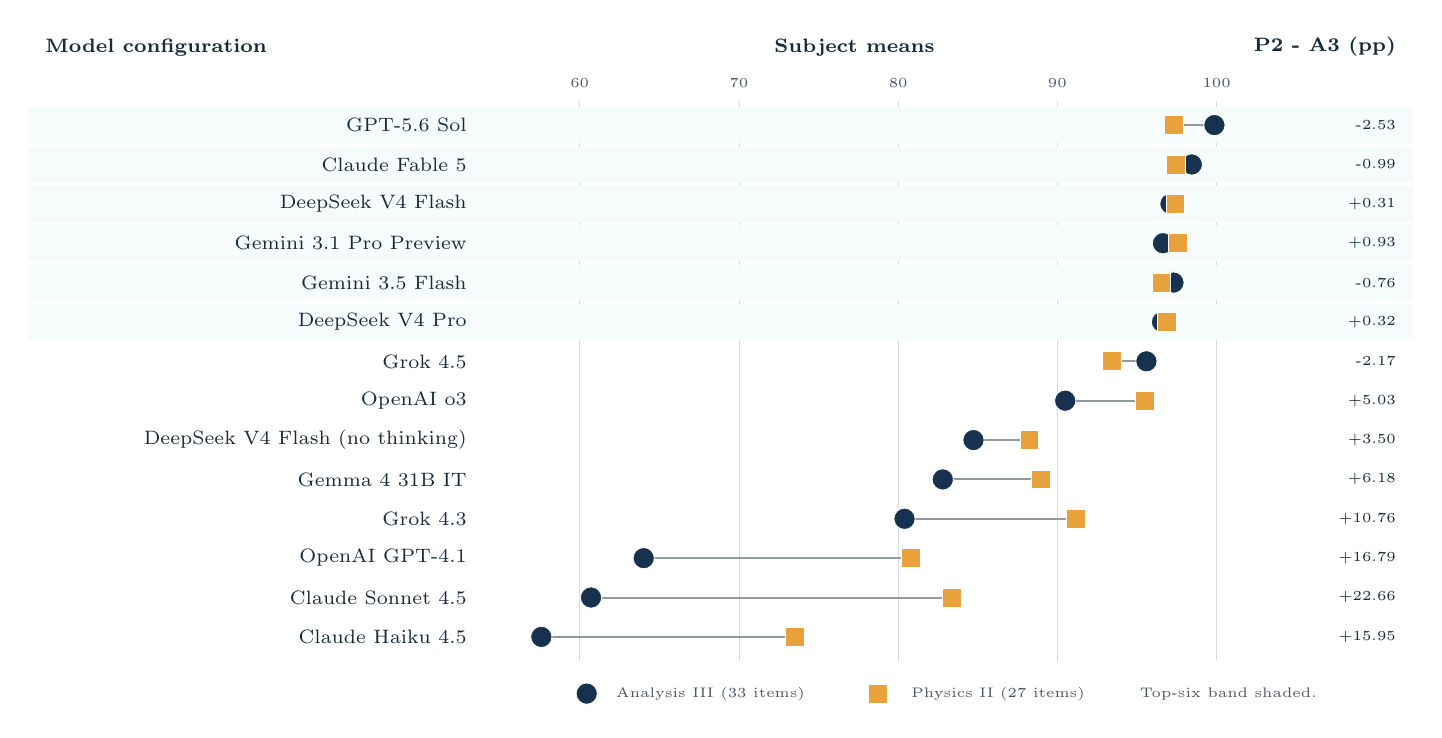
\begin{tikzpicture}[x=1mm,y=1mm,font=\scriptsize]
  \def\plotleft{-28}
  \def\plotwidth{91}
  \newcount\subjectrowcount
  \subjectrowcount=0

  \foreach \tick in {60,70,80,90,100}{
    \pgfmathsetmacro{\xtick}{\plotleft+(\tick-55)*\plotwidth/45}
    \draw[rulegray!48,line width=0.25pt] (\xtick,3) -- (\xtick,-68);
    \node[font=\tiny,text=darkgray,anchor=south] at (\xtick,3.5) {\tick};
  }
  \node[font=\scriptsize\bfseries,anchor=south west,text=ink] at (-87,7.5)
    {Model configuration};
  \node[font=\scriptsize\bfseries,anchor=south,text=ink] at (17,7.5)
    {Subject means};
  \node[font=\scriptsize\bfseries,anchor=south east,text=ink] at (87,7.5)
    {P2 - A3 (pp)};

  \newcommand{\subjectrow}[4]{%
    \pgfmathsetmacro{\yy}{-5*\the\subjectrowcount}
    \ifnum\subjectrowcount<6
      \fill[cyan!4] (-88,\yy-2.25) rectangle (88,\yy+2.25);
    \fi
    \node[anchor=east,font=\scriptsize,text=ink] at (-31,\yy) {#1};
    \pgfmathsetmacro{\xa}{\plotleft+(#2-55)*\plotwidth/45}
    \pgfmathsetmacro{\xp}{\plotleft+(#3-55)*\plotwidth/45}
    \draw[darkgray!60,line width=0.75pt] (\xa,\yy) -- (\xp,\yy);
    \filldraw[fill=navy,draw=white,line width=0.3pt] (\xa,\yy) circle (1.35);
    \filldraw[fill=gold,draw=white,line width=0.3pt]
      (\xp-1.2,\yy-1.2) rectangle (\xp+1.2,\yy+1.2);
    \node[anchor=east,font=\tiny,text=ink] at (87,\yy) {#4};
    \advance\subjectrowcount by 1
  }

  \subjectrow{GPT-5.6 Sol}{99.86}{97.33}{-2.53}
  \subjectrow{Claude Fable 5}{98.44}{97.45}{-0.99}
  \subjectrow{DeepSeek V4 Flash}{97.10}{97.41}{+0.31}
  \subjectrow{Gemini 3.1 Pro Preview}{96.63}{97.56}{+0.93}
  \subjectrow{Gemini 3.5 Flash}{97.29}{96.53}{-0.76}
  \subjectrow{DeepSeek V4 Pro}{96.57}{96.89}{+0.32}
  \subjectrow{Grok 4.5}{95.59}{93.42}{-2.17}
  \subjectrow{OpenAI o3}{90.49}{95.52}{+5.03}
  \subjectrow{DeepSeek V4 Flash (no thinking)}{84.73}{88.24}{+3.50}
  \subjectrow{Gemma 4 31B IT}{82.80}{88.98}{+6.18}
  \subjectrow{Grok 4.3}{80.40}{91.16}{+10.76}
  \subjectrow{OpenAI GPT-4.1}{64.02}{80.82}{+16.79}
  \subjectrow{Claude Sonnet 4.5}{60.71}{83.37}{+22.66}
  \subjectrow{Claude Haiku 4.5}{57.59}{73.54}{+15.95}

  \filldraw[fill=navy,draw=white,line width=0.3pt] (-17,-72.2) circle (1.35);
  \node[font=\tiny,anchor=west,text=darkgray] at (-14.5,-72.2) {Analysis III (33 items)};
  \filldraw[fill=gold,draw=white,line width=0.3pt]
    (18.8,-73.4) rectangle (21.2,-71.0);
  \node[font=\tiny,anchor=west,text=darkgray] at (23,-72.2) {Physics II (27 items)};
  \node[font=\tiny,anchor=west,text=darkgray] at (52,-72.2) {Top-six band shaded.};
\end{tikzpicture}
}
\caption{Cross-domain score heterogeneity. Subject means and their paired
difference are reported on a common scale; because the two subjects contain
different exercises, the gaps are descriptive domain contrasts rather than
causal estimates of subject difficulty.}
\label{fig:subjects}
\end{figure*}

The dimension panel in \cref{fig:performance} identifies what the scalar score
hides. Results and coverage (T4) is the weakest fully comparable dimension in
both subjects. The common residual weakness is therefore not merely selecting
a method; it is carrying the response through every requested result. T8 is
shown separately because its restricted 14-item denominator is not comparable
with the populations used for T1--T7.

The current judgment ledger records 1,211 atomic errors across 508 retained
responses, predominantly at major severity. Because these counts are
response-level, replicated cells receive more weight and the ledger is not used
to rank models. Raw category labels are also not yet a controlled taxonomy.
Severity and the frozen T1--T8 mapping are the defensible aggregate views; ad
hoc frequency claims from synonymous category strings are avoided.

The paired view in \cref{fig:subjects} shows that the leading configurations
remain stable across subjects, whereas several lower-ranked systems perform
substantially better in Physics II than in Analysis III. This domain
sensitivity would be obscured by separate subject rankings.

\subsection{Reasoning is valuable, but not free}

DeepSeek V4 Flash is the cleanest configuration contrast because the API
identifier, weights, prompt, and 60 items are held fixed while thinking is
toggled. High reasoning raises the score from 86.31\% to 97.24\%, a paired
gain of 10.93 pp (95\% CI 7.97--14.10), while substantially reducing the share
of responses containing a recorded atomic error.

The resource changes in \cref{fig:ablation} show that the gain requires more
than three times the token volume and estimated cost and more than five times
the median response time. Visible output nevertheless decreases, indicating
that the additional volume is internal reasoning rather than a longer displayed
derivation. The conclusion is configuration-specific: high reasoning is
decisive for this model on these tasks, but it shifts every measured resource
coordinate.

\begin{figure*}[!t]
\centering
\resizebox{0.95\textwidth}{!}{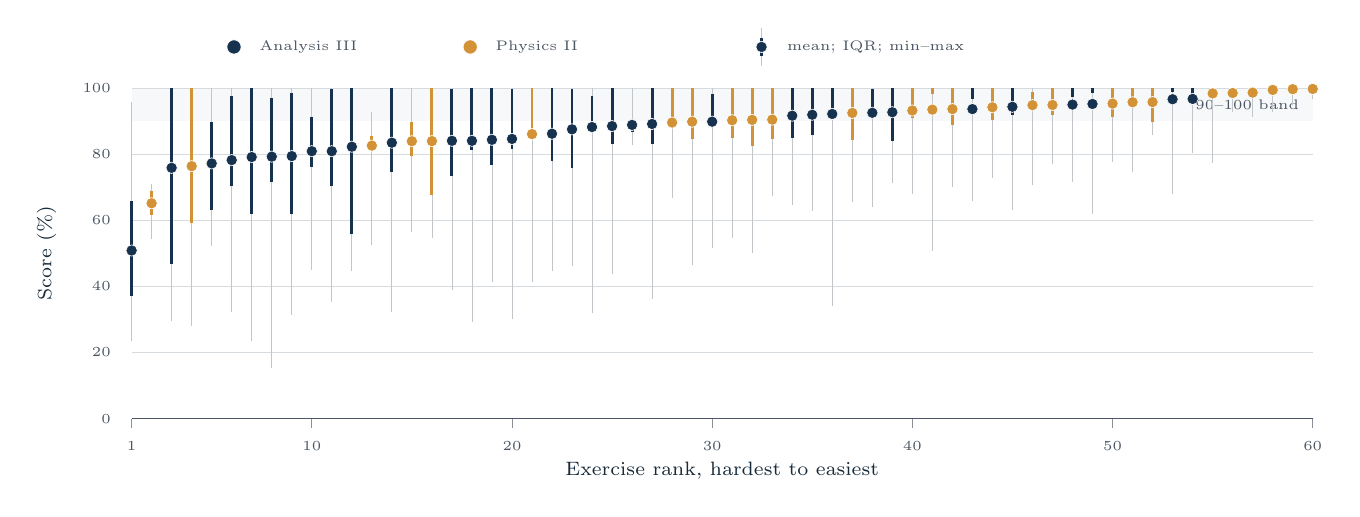
\begin{tikzpicture}[x=1mm,y=1mm,font=\scriptsize]
  \fill[lightgray!72] (12,37.8) rectangle (162,42);
  \node[font=\tiny,text=darkgray,anchor=east] at (161.5,39.9) {90--100 band};
  \draw[rulegray!48,line width=0.25pt] (12.00,0.00) -- (162.00,0.00);
  \node[font=\tiny,text=darkgray,anchor=east] at (10.60,0.00) {0};
  \draw[rulegray!48,line width=0.25pt] (12.00,8.40) -- (162.00,8.40);
  \node[font=\tiny,text=darkgray,anchor=east] at (10.60,8.40) {20};
  \draw[rulegray!48,line width=0.25pt] (12.00,16.80) -- (162.00,16.80);
  \node[font=\tiny,text=darkgray,anchor=east] at (10.60,16.80) {40};
  \draw[rulegray!48,line width=0.25pt] (12.00,25.20) -- (162.00,25.20);
  \node[font=\tiny,text=darkgray,anchor=east] at (10.60,25.20) {60};
  \draw[rulegray!48,line width=0.25pt] (12.00,33.60) -- (162.00,33.60);
  \node[font=\tiny,text=darkgray,anchor=east] at (10.60,33.60) {80};
  \draw[rulegray!48,line width=0.25pt] (12.00,42.00) -- (162.00,42.00);
  \node[font=\tiny,text=darkgray,anchor=east] at (10.60,42.00) {100};
  \draw[darkgray!65,line width=0.35pt] (12.00,0) -- (12.00,-1.15);
  \node[font=\tiny,text=darkgray,anchor=north] at (12.00,-1.65) {1};
  \draw[darkgray!65,line width=0.35pt] (34.88,0) -- (34.88,-1.15);
  \node[font=\tiny,text=darkgray,anchor=north] at (34.88,-1.65) {10};
  \draw[darkgray!65,line width=0.35pt] (60.31,0) -- (60.31,-1.15);
  \node[font=\tiny,text=darkgray,anchor=north] at (60.31,-1.65) {20};
  \draw[darkgray!65,line width=0.35pt] (85.73,0) -- (85.73,-1.15);
  \node[font=\tiny,text=darkgray,anchor=north] at (85.73,-1.65) {30};
  \draw[darkgray!65,line width=0.35pt] (111.15,0) -- (111.15,-1.15);
  \node[font=\tiny,text=darkgray,anchor=north] at (111.15,-1.65) {40};
  \draw[darkgray!65,line width=0.35pt] (136.58,0) -- (136.58,-1.15);
  \node[font=\tiny,text=darkgray,anchor=north] at (136.58,-1.65) {50};
  \draw[darkgray!65,line width=0.35pt] (162.00,0) -- (162.00,-1.15);
  \node[font=\tiny,text=darkgray,anchor=north] at (162.00,-1.65) {60};
  \draw[darkgray!34,line width=0.28pt] (12.00,9.87) -- (12.00,40.25);
  \draw[navy,line width=1.05pt] (12.00,15.59) -- (12.00,27.61);
  \filldraw[fill=navy,draw=white,line width=0.22pt] (12.00,21.35) circle (0.72);
  \draw[darkgray!34,line width=0.28pt] (14.54,22.77) -- (14.54,29.84);
  \draw[gold!90!black,line width=1.05pt] (14.54,25.81) -- (14.54,28.93);
  \filldraw[fill=gold!90!black,draw=white,line width=0.22pt] (14.54,27.35) circle (0.72);
  \draw[darkgray!34,line width=0.28pt] (17.08,12.39) -- (17.08,42.00);
  \draw[navy,line width=1.05pt] (17.08,19.64) -- (17.08,42.00);
  \filldraw[fill=navy,draw=white,line width=0.22pt] (17.08,31.85) circle (0.72);
  \draw[darkgray!34,line width=0.28pt] (19.63,11.72) -- (19.63,42.00);
  \draw[gold!90!black,line width=1.05pt] (19.63,24.87) -- (19.63,42.00);
  \filldraw[fill=gold!90!black,draw=white,line width=0.22pt] (19.63,32.06) circle (0.72);
  \draw[darkgray!34,line width=0.28pt] (22.17,21.95) -- (22.17,42.00);
  \draw[navy,line width=1.05pt] (22.17,26.46) -- (22.17,37.70);
  \filldraw[fill=navy,draw=white,line width=0.22pt] (22.17,32.41) circle (0.72);
  \draw[darkgray!34,line width=0.28pt] (24.71,13.48) -- (24.71,42.00);
  \draw[navy,line width=1.05pt] (24.71,29.48) -- (24.71,41.01);
  \filldraw[fill=navy,draw=white,line width=0.22pt] (24.71,32.83) circle (0.72);
  \draw[darkgray!34,line width=0.28pt] (27.25,9.87) -- (27.25,42.00);
  \draw[navy,line width=1.05pt] (27.25,25.93) -- (27.25,42.00);
  \filldraw[fill=navy,draw=white,line width=0.22pt] (27.25,33.22) circle (0.72);
  \draw[darkgray!34,line width=0.28pt] (29.80,6.41) -- (29.80,42.00);
  \draw[navy,line width=1.05pt] (29.80,30.09) -- (29.80,40.70);
  \filldraw[fill=navy,draw=white,line width=0.22pt] (29.80,33.27) circle (0.72);
  \draw[darkgray!34,line width=0.28pt] (32.34,13.12) -- (32.34,42.00);
  \draw[navy,line width=1.05pt] (32.34,25.99) -- (32.34,41.29);
  \filldraw[fill=navy,draw=white,line width=0.22pt] (32.34,33.34) circle (0.72);
  \draw[darkgray!34,line width=0.28pt] (34.88,18.90) -- (34.88,42.00);
  \draw[navy,line width=1.05pt] (34.88,32.00) -- (34.88,38.33);
  \filldraw[fill=navy,draw=white,line width=0.22pt] (34.88,33.96) circle (0.72);
  \draw[darkgray!34,line width=0.28pt] (37.42,14.80) -- (37.42,42.00);
  \draw[navy,line width=1.05pt] (37.42,29.48) -- (37.42,41.87);
  \filldraw[fill=navy,draw=white,line width=0.22pt] (37.42,33.96) circle (0.72);
  \draw[darkgray!34,line width=0.28pt] (39.97,18.69) -- (39.97,42.00);
  \draw[navy,line width=1.05pt] (39.97,23.41) -- (39.97,42.00);
  \filldraw[fill=navy,draw=white,line width=0.22pt] (39.97,34.53) circle (0.72);
  \draw[darkgray!34,line width=0.28pt] (42.51,22.11) -- (42.51,38.91);
  \draw[gold!90!black,line width=1.05pt] (42.51,34.65) -- (42.51,35.95);
  \filldraw[fill=gold!90!black,draw=white,line width=0.22pt] (42.51,34.67) circle (0.72);
  \draw[darkgray!34,line width=0.28pt] (45.05,13.54) -- (45.05,42.00);
  \draw[navy,line width=1.05pt] (45.05,31.37) -- (45.05,42.00);
  \filldraw[fill=navy,draw=white,line width=0.22pt] (45.05,35.04) circle (0.72);
  \draw[darkgray!34,line width=0.28pt] (47.59,23.76) -- (47.59,42.00);
  \draw[gold!90!black,line width=1.05pt] (47.59,33.38) -- (47.59,37.72);
  \filldraw[fill=gold!90!black,draw=white,line width=0.22pt] (47.59,35.23) circle (0.72);
  \draw[darkgray!34,line width=0.28pt] (50.14,22.88) -- (50.14,42.00);
  \draw[gold!90!black,line width=1.05pt] (50.14,28.38) -- (50.14,42.00);
  \filldraw[fill=gold!90!black,draw=white,line width=0.22pt] (50.14,35.24) circle (0.72);
  \draw[darkgray!34,line width=0.28pt] (52.68,16.38) -- (52.68,42.00);
  \draw[navy,line width=1.05pt] (52.68,30.77) -- (52.68,41.90);
  \filldraw[fill=navy,draw=white,line width=0.22pt] (52.68,35.28) circle (0.72);
  \draw[darkgray!34,line width=0.28pt] (55.22,12.27) -- (55.22,42.00);
  \draw[navy,line width=1.05pt] (55.22,34.12) -- (55.22,42.00);
  \filldraw[fill=navy,draw=white,line width=0.22pt] (55.22,35.28) circle (0.72);
  \draw[darkgray!34,line width=0.28pt] (57.76,17.35) -- (57.76,42.00);
  \draw[navy,line width=1.05pt] (57.76,32.19) -- (57.76,42.00);
  \filldraw[fill=navy,draw=white,line width=0.22pt] (57.76,35.41) circle (0.72);
  \draw[darkgray!34,line width=0.28pt] (60.31,12.60) -- (60.31,42.00);
  \draw[navy,line width=1.05pt] (60.31,34.26) -- (60.31,41.84);
  \filldraw[fill=navy,draw=white,line width=0.22pt] (60.31,35.52) circle (0.72);
  \draw[darkgray!34,line width=0.28pt] (62.85,17.35) -- (62.85,42.00);
  \draw[gold!90!black,line width=1.05pt] (62.85,36.23) -- (62.85,42.00);
  \filldraw[fill=gold!90!black,draw=white,line width=0.22pt] (62.85,36.13) circle (0.72);
  \draw[darkgray!34,line width=0.28pt] (65.39,18.69) -- (65.39,42.00);
  \draw[navy,line width=1.05pt] (65.39,32.77) -- (65.39,42.00);
  \filldraw[fill=navy,draw=white,line width=0.22pt] (65.39,36.18) circle (0.72);
  \draw[darkgray!34,line width=0.28pt] (67.93,19.34) -- (67.93,42.00);
  \draw[navy,line width=1.05pt] (67.93,31.80) -- (67.93,41.89);
  \filldraw[fill=navy,draw=white,line width=0.22pt] (67.93,36.74) circle (0.72);
  \draw[darkgray!34,line width=0.28pt] (70.47,13.37) -- (70.47,42.00);
  \draw[navy,line width=1.05pt] (70.47,36.92) -- (70.47,41.01);
  \filldraw[fill=navy,draw=white,line width=0.22pt] (70.47,37.03) circle (0.72);
  \draw[darkgray!34,line width=0.28pt] (73.02,18.35) -- (73.02,42.00);
  \draw[navy,line width=1.05pt] (73.02,34.93) -- (73.02,42.00);
  \filldraw[fill=navy,draw=white,line width=0.22pt] (73.02,37.15) circle (0.72);
  \draw[darkgray!34,line width=0.28pt] (75.56,34.71) -- (75.56,42.00);
  \draw[navy,line width=1.05pt] (75.56,36.42) -- (75.56,37.80);
  \filldraw[fill=navy,draw=white,line width=0.22pt] (75.56,37.30) circle (0.72);
  \draw[darkgray!34,line width=0.28pt] (78.10,15.14) -- (78.10,42.00);
  \draw[navy,line width=1.05pt] (78.10,34.93) -- (78.10,42.00);
  \filldraw[fill=navy,draw=white,line width=0.22pt] (78.10,37.42) circle (0.72);
  \draw[darkgray!34,line width=0.28pt] (80.64,27.96) -- (80.64,42.00);
  \draw[gold!90!black,line width=1.05pt] (80.64,37.33) -- (80.64,42.00);
  \filldraw[fill=gold!90!black,draw=white,line width=0.22pt] (80.64,37.60) circle (0.72);
  \draw[darkgray!34,line width=0.28pt] (83.19,19.45) -- (83.19,42.00);
  \draw[gold!90!black,line width=1.05pt] (83.19,35.45) -- (83.19,42.00);
  \filldraw[fill=gold!90!black,draw=white,line width=0.22pt] (83.19,37.71) circle (0.72);
  \draw[darkgray!34,line width=0.28pt] (85.73,21.66) -- (85.73,42.00);
  \draw[navy,line width=1.05pt] (85.73,37.36) -- (85.73,41.23);
  \filldraw[fill=navy,draw=white,line width=0.22pt] (85.73,37.71) circle (0.72);
  \draw[darkgray!34,line width=0.28pt] (88.27,22.99) -- (88.27,42.00);
  \draw[gold!90!black,line width=1.05pt] (88.27,35.64) -- (88.27,42.00);
  \filldraw[fill=gold!90!black,draw=white,line width=0.22pt] (88.27,37.89) circle (0.72);
  \draw[darkgray!34,line width=0.28pt] (90.81,21.00) -- (90.81,42.00);
  \draw[gold!90!black,line width=1.05pt] (90.81,34.65) -- (90.81,42.00);
  \filldraw[fill=gold!90!black,draw=white,line width=0.22pt] (90.81,37.94) circle (0.72);
  \draw[darkgray!34,line width=0.28pt] (93.36,28.29) -- (93.36,42.00);
  \draw[gold!90!black,line width=1.05pt] (93.36,35.51) -- (93.36,42.00);
  \filldraw[fill=gold!90!black,draw=white,line width=0.22pt] (93.36,37.97) circle (0.72);
  \draw[darkgray!34,line width=0.28pt] (95.90,27.08) -- (95.90,42.00);
  \draw[navy,line width=1.05pt] (95.90,35.67) -- (95.90,42.00);
  \filldraw[fill=navy,draw=white,line width=0.22pt] (95.90,38.47) circle (0.72);
  \draw[darkgray!34,line width=0.28pt] (98.44,26.31) -- (98.44,42.00);
  \draw[navy,line width=1.05pt] (98.44,35.98) -- (98.44,42.00);
  \filldraw[fill=navy,draw=white,line width=0.22pt] (98.44,38.59) circle (0.72);
  \draw[darkgray!34,line width=0.28pt] (100.98,14.26) -- (100.98,42.00);
  \draw[navy,line width=1.05pt] (100.98,39.51) -- (100.98,42.00);
  \filldraw[fill=navy,draw=white,line width=0.22pt] (100.98,38.69) circle (0.72);
  \draw[darkgray!34,line width=0.28pt] (103.53,27.52) -- (103.53,42.00);
  \draw[gold!90!black,line width=1.05pt] (103.53,35.37) -- (103.53,42.00);
  \filldraw[fill=gold!90!black,draw=white,line width=0.22pt] (103.53,38.82) circle (0.72);
  \draw[darkgray!34,line width=0.28pt] (106.07,26.88) -- (106.07,42.00);
  \draw[navy,line width=1.05pt] (106.07,38.61) -- (106.07,41.90);
  \filldraw[fill=navy,draw=white,line width=0.22pt] (106.07,38.84) circle (0.72);
  \draw[darkgray!34,line width=0.28pt] (108.61,29.95) -- (108.61,42.00);
  \draw[navy,line width=1.05pt] (108.61,35.31) -- (108.61,42.00);
  \filldraw[fill=navy,draw=white,line width=0.22pt] (108.61,38.91) circle (0.72);
  \draw[darkgray!34,line width=0.28pt] (111.15,28.52) -- (111.15,42.00);
  \draw[gold!90!black,line width=1.05pt] (111.15,38.24) -- (111.15,42.00);
  \filldraw[fill=gold!90!black,draw=white,line width=0.22pt] (111.15,39.13) circle (0.72);
  \draw[darkgray!34,line width=0.28pt] (113.69,21.33) -- (113.69,42.00);
  \draw[gold!90!black,line width=1.05pt] (113.69,41.23) -- (113.69,42.00);
  \filldraw[fill=gold!90!black,draw=white,line width=0.22pt] (113.69,39.24) circle (0.72);
  \draw[darkgray!34,line width=0.28pt] (116.24,29.40) -- (116.24,42.00);
  \draw[gold!90!black,line width=1.05pt] (116.24,37.33) -- (116.24,42.00);
  \filldraw[fill=gold!90!black,draw=white,line width=0.22pt] (116.24,39.31) circle (0.72);
  \draw[darkgray!34,line width=0.28pt] (118.78,27.63) -- (118.78,42.00);
  \draw[navy,line width=1.05pt] (118.78,40.59) -- (118.78,42.00);
  \filldraw[fill=navy,draw=white,line width=0.22pt] (118.78,39.31) circle (0.72);
  \draw[darkgray!34,line width=0.28pt] (121.32,30.62) -- (121.32,42.00);
  \draw[gold!90!black,line width=1.05pt] (121.32,37.88) -- (121.32,42.00);
  \filldraw[fill=gold!90!black,draw=white,line width=0.22pt] (121.32,39.54) circle (0.72);
  \draw[darkgray!34,line width=0.28pt] (123.86,26.53) -- (123.86,42.00);
  \draw[navy,line width=1.05pt] (123.86,38.55) -- (123.86,42.00);
  \filldraw[fill=navy,draw=white,line width=0.22pt] (123.86,39.60) circle (0.72);
  \draw[darkgray!34,line width=0.28pt] (126.41,29.62) -- (126.41,42.00);
  \draw[gold!90!black,line width=1.05pt] (126.41,39.73) -- (126.41,41.45);
  \filldraw[fill=gold!90!black,draw=white,line width=0.22pt] (126.41,39.81) circle (0.72);
  \draw[darkgray!34,line width=0.28pt] (128.95,32.38) -- (128.95,42.00);
  \draw[gold!90!black,line width=1.05pt] (128.95,38.55) -- (128.95,42.00);
  \filldraw[fill=gold!90!black,draw=white,line width=0.22pt] (128.95,39.83) circle (0.72);
  \draw[darkgray!34,line width=0.28pt] (131.49,30.06) -- (131.49,42.00);
  \draw[navy,line width=1.05pt] (131.49,40.81) -- (131.49,42.00);
  \filldraw[fill=navy,draw=white,line width=0.22pt] (131.49,39.88) circle (0.72);
  \draw[darkgray!34,line width=0.28pt] (134.03,26.04) -- (134.03,42.00);
  \draw[navy,line width=1.05pt] (134.03,41.37) -- (134.03,42.00);
  \filldraw[fill=navy,draw=white,line width=0.22pt] (134.03,39.96) circle (0.72);
  \draw[darkgray!34,line width=0.28pt] (136.58,32.61) -- (136.58,42.00);
  \draw[gold!90!black,line width=1.05pt] (136.58,38.30) -- (136.58,42.00);
  \filldraw[fill=gold!90!black,draw=white,line width=0.22pt] (136.58,40.01) circle (0.72);
  \draw[darkgray!34,line width=0.28pt] (139.12,31.28) -- (139.12,42.00);
  \draw[gold!90!black,line width=1.05pt] (139.12,39.76) -- (139.12,42.00);
  \filldraw[fill=gold!90!black,draw=white,line width=0.22pt] (139.12,40.18) circle (0.72);
  \draw[darkgray!34,line width=0.28pt] (141.66,36.03) -- (141.66,42.00);
  \draw[gold!90!black,line width=1.05pt] (141.66,37.63) -- (141.66,42.00);
  \filldraw[fill=gold!90!black,draw=white,line width=0.22pt] (141.66,40.20) circle (0.72);
  \draw[darkgray!34,line width=0.28pt] (144.20,28.52) -- (144.20,42.00);
  \draw[navy,line width=1.05pt] (144.20,41.50) -- (144.20,42.00);
  \filldraw[fill=navy,draw=white,line width=0.22pt] (144.20,40.56) circle (0.72);
  \draw[darkgray!34,line width=0.28pt] (146.75,33.70) -- (146.75,42.00);
  \draw[navy,line width=1.05pt] (146.75,41.05) -- (146.75,42.00);
  \filldraw[fill=navy,draw=white,line width=0.22pt] (146.75,40.60) circle (0.72);
  \draw[darkgray!34,line width=0.28pt] (149.29,32.49) -- (149.29,42.00);
  \draw[gold!90!black,line width=1.05pt] (149.29,42.00) -- (149.29,42.00);
  \filldraw[fill=gold!90!black,draw=white,line width=0.22pt] (149.29,41.30) circle (0.72);
  \draw[darkgray!34,line width=0.28pt] (151.83,38.91) -- (151.83,42.00);
  \draw[gold!90!black,line width=1.05pt] (151.83,41.56) -- (151.83,41.56);
  \filldraw[fill=gold!90!black,draw=white,line width=0.22pt] (151.83,41.35) circle (0.72);
  \draw[darkgray!34,line width=0.28pt] (154.37,38.35) -- (154.37,42.00);
  \draw[gold!90!black,line width=1.05pt] (154.37,41.17) -- (154.37,42.00);
  \filldraw[fill=gold!90!black,draw=white,line width=0.22pt] (154.37,41.40) circle (0.72);
  \draw[darkgray!34,line width=0.28pt] (156.92,38.91) -- (156.92,42.00);
  \draw[gold!90!black,line width=1.05pt] (156.92,42.00) -- (156.92,42.00);
  \filldraw[fill=gold!90!black,draw=white,line width=0.22pt] (156.92,41.74) circle (0.72);
  \draw[darkgray!34,line width=0.28pt] (159.46,39.79) -- (159.46,42.00);
  \draw[gold!90!black,line width=1.05pt] (159.46,42.00) -- (159.46,42.00);
  \filldraw[fill=gold!90!black,draw=white,line width=0.22pt] (159.46,41.84) circle (0.72);
  \draw[darkgray!34,line width=0.28pt] (162.00,40.56) -- (162.00,42.00);
  \draw[gold!90!black,line width=1.05pt] (162.00,42.00) -- (162.00,42.00);
  \filldraw[fill=gold!90!black,draw=white,line width=0.22pt] (162.00,41.87) circle (0.72);
  \draw[darkgray,line width=0.45pt] (12,0) -- (162,0);
  \node[font=\scriptsize,rotate=90,text=ink] at (1.2,21) {Score (\%)};
  \node[font=\scriptsize,text=ink] at (87,-6.6) {Exercise rank, hardest to easiest};
  \filldraw[fill=navy,draw=white,line width=0.22pt] (25,47.2) circle (0.9);
  \node[font=\tiny,text=darkgray,anchor=west] at (27,47.2) {Analysis III};
  \filldraw[fill=gold!90!black,draw=white,line width=0.22pt] (55,47.2) circle (0.9);
  \node[font=\tiny,text=darkgray,anchor=west] at (57,47.2) {Physics II};
  \draw[darkgray!34,line width=0.28pt] (92,44.8) -- (92,49.6);
  \draw[navy,line width=1.05pt] (92,46.0) -- (92,48.4);
  \filldraw[fill=navy,draw=white,line width=0.22pt] (92,47.2) circle (0.72);
  \node[font=\tiny,text=darkgray,anchor=west] at (94,47.2) {mean; IQR; min--max};
\end{tikzpicture}
}
\caption{Difficulty profile of the 60 exercises. Items are ordered by their
mean score across the 14 configurations. Points mark means, thick segments the
interquartile range, and thin whiskers the full inter-model range; color denotes
subject. The shaded 90--100\% band makes the broad ceiling region visible while
retaining the smaller tail of strongly discriminating exercises.}
\label{fig:item-difficulty}
\end{figure*}

\begin{figure*}[!t]
\centering
\resizebox{0.95\textwidth}{!}{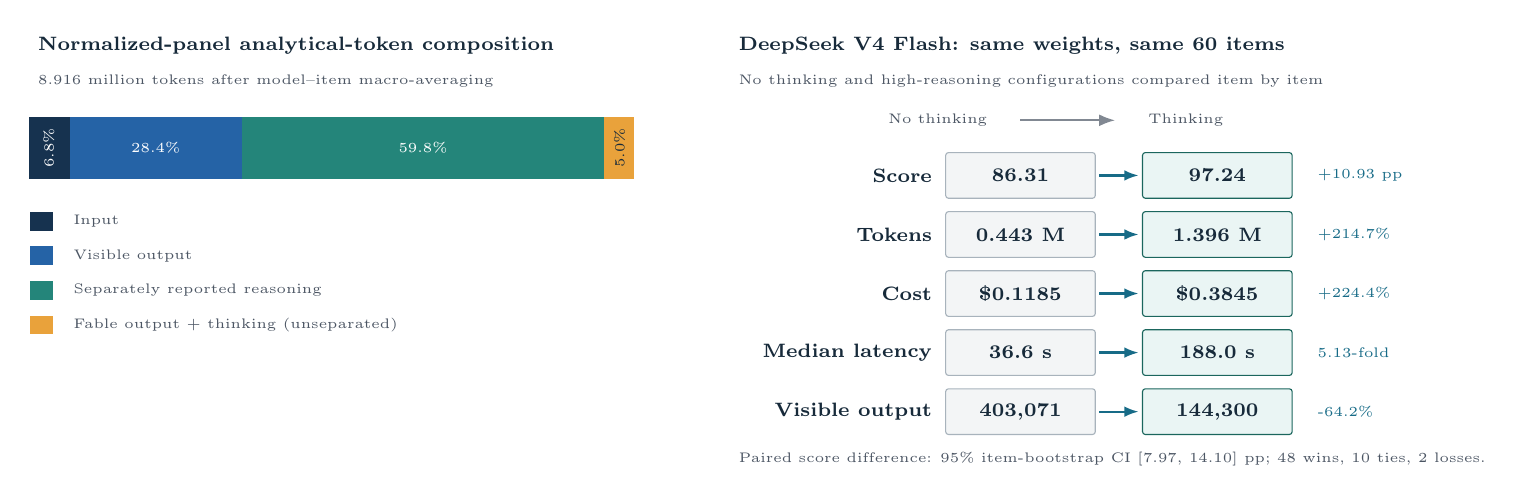
\begin{tikzpicture}[x=1mm,y=1mm,font=\scriptsize]
  % Left: aggregate analytical-token composition.
  \node[font=\scriptsize\bfseries,text=ink,anchor=west] at (-86,24)
    {Normalized-panel analytical-token composition};
  \node[font=\tiny,text=darkgray,anchor=west] at (-86,19.5)
    {8.916 million tokens after model--item macro-averaging};

  \def\barleft{-86}
  \def\barwidth{77}
  \pgfmathsetmacro{\a}{\barleft+0.06796*\barwidth}
  \pgfmathsetmacro{\b}{\a+0.28412*\barwidth}
  \pgfmathsetmacro{\c}{\b+0.59788*\barwidth}
  \pgfmathsetmacro{\midab}{0.5*(\a+\b)}
  \pgfmathsetmacro{\midbc}{0.5*(\b+\c)}
  \pgfmathsetmacro{\midclast}{0.5*(\c+\barleft+\barwidth)}
  \fill[navy] (\barleft,7) rectangle (\a,15);
  \fill[blue] (\a,7) rectangle (\b,15);
  \fill[cyan!85!black] (\b,7) rectangle (\c,15);
  \fill[gold] (\c,7) rectangle (\barleft+\barwidth,15);
  \draw[white,line width=0.5pt] (\barleft,7) rectangle (\barleft+\barwidth,15);
  \node[font=\tiny,text=white,rotate=90] at (\barleft+2.6,11) {6.8\%};
  \node[font=\tiny,text=white] at (\midab,11) {28.4\%};
  \node[font=\tiny,text=white] at (\midbc,11) {59.8\%};
  \node[font=\tiny,text=ink,rotate=90] at (\midclast,11) {5.0\%};

  \foreach \col/\lab/\yy in {navy/Input/1.7,blue/Visible output/-2.7,
    cyan!85!black/Separately reported reasoning/-7.1,gold/Fable output + thinking (unseparated)/-11.5}{
    \fill[\col] (-85.8,\yy-1.2) rectangle (-82.9,\yy+1.2);
    \node[font=\tiny,text=darkgray,anchor=west] at (-81.5,\yy) {\lab};
  }

  % Right: controlled DeepSeek thinking comparison.
  \node[font=\scriptsize\bfseries,text=ink,anchor=west] at (3,24)
    {DeepSeek V4 Flash: same weights, same 60 items};
  \node[font=\tiny,text=darkgray,anchor=west] at (3,19.5)
    {No thinking and high-reasoning configurations compared item by item};

  \node[font=\tiny,text=darkgray,anchor=east] at (37,14.5) {No thinking};
  \node[font=\tiny,text=darkgray,anchor=west] at (55,14.5) {Thinking};
  \draw[-{Latex[length=2mm]},darkgray!70,line width=0.6pt] (40,14.5) -- (52,14.5);

  \newcommand{\pairmetric}[5]{%
    \node[font=\scriptsize\bfseries,text=ink,anchor=east] at (30,#1) {#2};
    \node[rounded corners=1pt,fill=notegray,draw=rulegray,minimum width=19mm,
      minimum height=5.8mm,font=\scriptsize\bfseries,text=ink] at (40,#1) {#3};
    \draw[-{Latex[length=1.8mm]},accent,line width=0.8pt] (50,#1) -- (55,#1);
    \node[rounded corners=1pt,fill=cyan!10,draw=cyan!65!black,minimum width=19mm,
      minimum height=5.8mm,font=\scriptsize\bfseries,text=ink] at (65,#1) {#4};
    \node[font=\tiny,text=accent,anchor=west] at (76.5,#1) {#5};
  }
  \pairmetric{7.5}{Score}{86.31}{97.24}{+10.93 pp}
  \pairmetric{0}{Tokens}{0.443 M}{1.396 M}{+214.7\%}
  \pairmetric{-7.5}{Cost}{\$0.1185}{\$0.3845}{+224.4\%}
  \pairmetric{-15}{Median latency}{36.6 s}{188.0 s}{5.13-fold}
  \pairmetric{-22.5}{Visible output}{403,071}{144,300}{-64.2\%}

  \node[font=\tiny,text=darkgray,anchor=west] at (3,-28.5)
    {Paired score difference: 95\% item-bootstrap CI [7.97, 14.10] pp; 48 wins, 10 ties, 2 losses.};
\end{tikzpicture}
}
\caption{Token accounting and the DeepSeek thinking contrast. Left: aggregate
token composition; Fable output and hidden thinking are inseparable in the
available provider field. Right: paired same-weights comparison; the score
interval resamples items, whereas resource deltas are configuration-specific
summaries.}
\label{fig:ablation}
\end{figure*}

\subsection{Quality--resource frontiers}

After within-cell averaging, the matched comparison panel represents 8,915,801
analytical tokens and an estimated normalized cost of \$84.21. These are
equal-weight comparison totals, not a provider bill: before averaging, the 924
retained successful responses correspond to 10,054,390 analytical tokens and
an estimated \$105.10. Input accounts for 6.80\% of normalized volume, visible output 28.41\%, separately reported reasoning
59.79\%, and Fable's inseparable output/thinking field 5.00\%; model totals span
6.91-fold. Non-zero normalized model cost spans \$0.1185--\$27.8053
(234.61-fold), and GPT-5.6 Sol plus Fable account for 60.24\% of the normalized
comparison cost. Token volume and
price are only weakly associated (Spearman $\rho=0.23$), reflecting
provider-specific rate structures.

Median response time varies 12.46-fold; GPT-5.6 Sol is the slowest configuration
by this measure, at 307.05 seconds. Across the 14 models, score is associated
with log median latency (Pearson $r=0.80$; Spearman $\rho=0.78$), but this
small-sample relationship is neither item-level nor causal. Gemini 3.5 Flash
and Fable are operationally important exceptions, combining near-ceiling scores
with markedly lower medians. Retry-heavy tails also make means less
representative for several configurations.

\begin{figure*}[!t]
\centering
\resizebox{0.98\textwidth}{!}{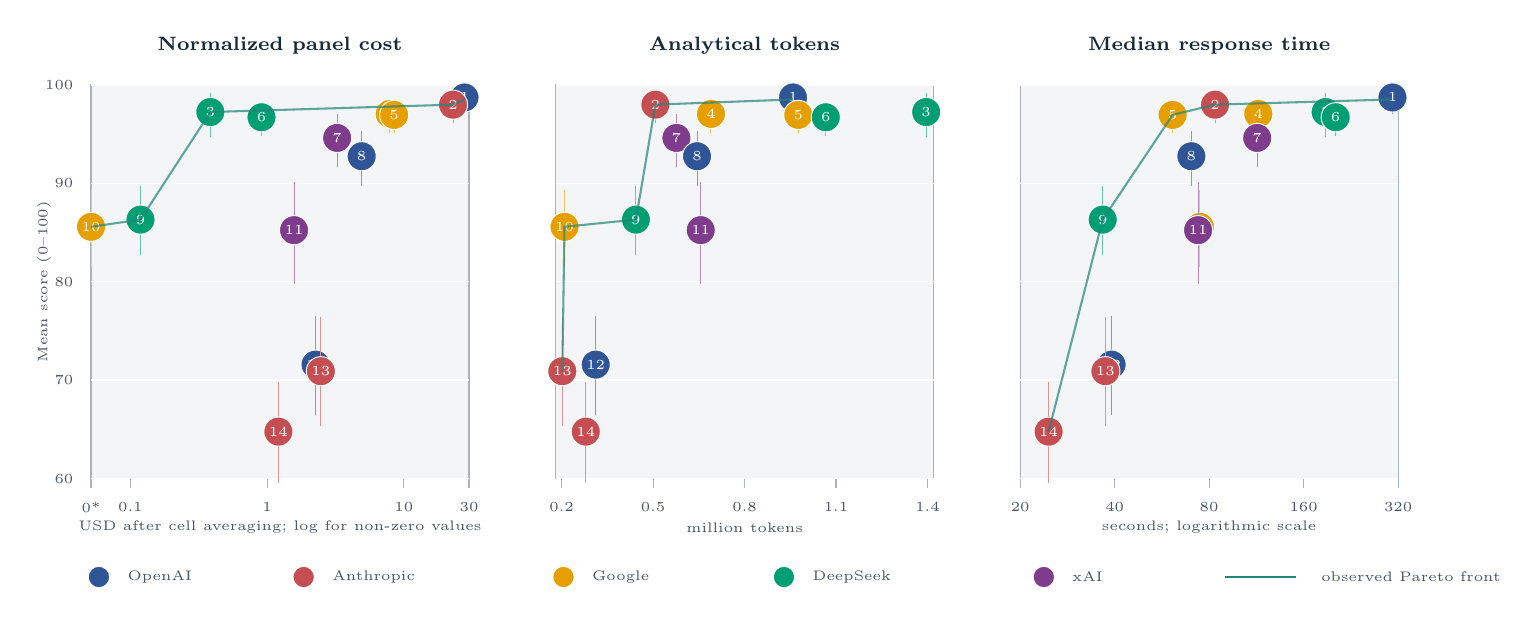
\begin{tikzpicture}[x=1mm,y=1mm,font=\scriptsize]
  \def\costx{-84}
  \def\tokenx{-25}
  \def\timex{34}
  \def\ybase{-24}
  \def\panelw{48}

  % Shared panel backgrounds and score grid.
  \foreach \xx/\title in {\costx/{Normalized panel cost},\tokenx/{Analytical tokens},\timex/{Median response time}}{
    \fill[notegray] (\xx,\ybase) rectangle (\xx+\panelw,\ybase+50);
    \draw[rulegray,line width=0.4pt] (\xx,\ybase) rectangle (\xx+\panelw,\ybase+50);
    \node[font=\scriptsize\bfseries,text=ink] at (\xx+24,31) {\title};
    \foreach \sc in {60,70,80,90,100}{
      \pgfmathsetmacro{\yy}{\ybase+(\sc-60)*1.25}
      \draw[white,line width=0.55pt] (\xx,\yy) -- (\xx+\panelw,\yy);
    }
  }
  \node[font=\tiny,text=darkgray,rotate=90] at (-90,1) {Mean score (0--100)};
  \foreach \sc in {60,70,80,90,100}{
    \pgfmathsetmacro{\yy}{\ybase+(\sc-60)*1.25}
    \node[font=\tiny,text=darkgray,anchor=east] at (-85,\yy) {\sc};
  }

  % X ticks. Cost uses a separate zero point and a log scale for non-zero values.
  \foreach \x/\lab in {0/{0*},5/{0.1},22.36/{1},39.72/{10},48/{30}}{
    \draw[rulegray] (\costx+\x,\ybase) -- (\costx+\x,\ybase-1.2);
    \node[font=\tiny,text=darkgray,anchor=north] at (\costx+\x,\ybase-1.8) {\lab};
  }
  \node[font=\tiny,text=darkgray] at (\costx+24,-30.2) {USD after cell averaging; log for non-zero values};
  \foreach \x/\lab in {0.77/{0.2},12.39/{0.5},24/{0.8},35.61/{1.1},47.23/{1.4}}{
    \draw[rulegray] (\tokenx+\x,\ybase) -- (\tokenx+\x,\ybase-1.2);
    \node[font=\tiny,text=darkgray,anchor=north] at (\tokenx+\x,\ybase-1.8) {\lab};
  }
  \node[font=\tiny,text=darkgray] at (\tokenx+24,-30.2) {million tokens};
  \foreach \x/\lab in {0/{20},12/{40},24/{80},36/{160},48/{320}}{
    \draw[rulegray] (\timex+\x,\ybase) -- (\timex+\x,\ybase-1.2);
    \node[font=\tiny,text=darkgray,anchor=north] at (\timex+\x,\ybase-1.8) {\lab};
  }
  \node[font=\tiny,text=darkgray] at (\timex+24,-30.2) {seconds; logarithmic scale};

  \newcommand{\resrow}[8]{%
    \pgfmathsetmacro{\ym}{\ybase+(#3-60)*1.25}
    \pgfmathsetmacro{\yl}{\ybase+(#4-60)*1.25}
    \pgfmathsetmacro{\yh}{\ybase+(#5-60)*1.25}
    \foreach \origin/\xx in {\costx/#6,\tokenx/#7,\timex/#8}{
      \draw[#2!60,line width=0.35pt] (\origin+\xx,\yl) -- (\origin+\xx,\yh);
      \node[circle,fill=#2,draw=white,line width=0.35pt,inner sep=0pt,
            minimum size=3.7mm,font=\tiny,text=white]
        at (\origin+\xx,\ym) {#1};
    }
  }

  \resrow{1}{openaiC}{98.72}{97.04}{99.86}{47.43}{30.15}{47.28}
  \resrow{2}{anthropicC}{97.99}{96.15}{99.38}{45.97}{12.67}{24.74}
  \resrow{3}{deepseekC}{97.24}{94.66}{99.16}{15.15}{47.06}{38.79}
  \resrow{4}{googleC}{97.05}{95.11}{98.60}{37.93}{19.73}{30.24}
  \resrow{5}{googleC}{96.95}{95.10}{98.51}{38.49}{30.82}{19.36}
  \resrow{6}{deepseekC}{96.71}{94.76}{98.31}{21.65}{34.31}{40.07}
  \resrow{7}{xaiC}{94.61}{91.66}{97.08}{31.25}{15.34}{30.10}
  \resrow{8}{openaiC}{92.75}{89.74}{95.33}{34.37}{17.96}{21.74}
  \resrow{9}{deepseekC}{86.31}{82.73}{89.68}{6.28}{10.20}{10.48}
  \resrow{10}{googleC}{85.58}{81.52}{89.34}{0.00}{1.13}{22.83}
  \resrow{11}{xaiC}{85.24}{79.77}{90.11}{25.78}{18.43}{22.59}
  \resrow{12}{openaiC}{71.58}{66.46}{76.53}{28.51}{5.09}{11.61}
  \resrow{13}{anthropicC}{70.91}{65.31}{76.41}{29.18}{0.85}{10.82}
  \resrow{14}{anthropicC}{64.77}{59.57}{69.80}{23.79}{3.83}{3.61}

  % Observed two-dimensional Pareto fronts, drawn after points.
  \draw[cyan!85!black,line width=0.75pt,opacity=0.72]
    (\costx+0,7.98) -- (\costx+6.28,8.89) -- (\costx+15.15,22.55)
    -- (\costx+45.97,23.49) -- (\costx+47.43,24.15);
  \draw[cyan!85!black,line width=0.75pt,opacity=0.72]
    (\tokenx+0.85,-10.36) -- (\tokenx+1.13,7.98) -- (\tokenx+10.20,8.89)
    -- (\tokenx+12.67,23.49) -- (\tokenx+30.15,24.15);
  \draw[cyan!85!black,line width=0.75pt,opacity=0.72]
    (\timex+3.61,-18.04) -- (\timex+10.48,8.89) -- (\timex+19.36,22.19)
    -- (\timex+24.74,23.49) -- (\timex+47.28,24.15);

  % Legend and interpretation key.
  \foreach \col/\lab/\x in {openaiC/OpenAI/-83,anthropicC/Anthropic/-57,
    googleC/Google/-24,deepseekC/DeepSeek/4,xaiC/xAI/37}{
    \filldraw[fill=\col,draw=white,line width=0.3pt] (\x,-36.5) circle (1.35);
    \node[font=\tiny,anchor=west,text=darkgray] at (\x+2.4,-36.5) {\lab};
  }
  \draw[cyan!85!black,line width=1.05pt] (60,-36.5) -- (69,-36.5);
  \node[font=\tiny,anchor=west,text=darkgray] at (71,-36.5) {observed Pareto front};
\end{tikzpicture}
}
\caption{Accuracy--resource views for the same 14 configurations. Point
numbers are ranks from \cref{tab:main-results}; vertical segments reproduce
score intervals. Cyan lines mark the observed two-dimensional Pareto fronts,
not fitted curves. The cost panel uses the normalized, cell-averaged estimates,
treats Gemma's campaign-specific zero as a separate point, and applies a
logarithmic scale only to non-zero values. A system
can be efficient in one panel and inefficient in another, so no composite
``winner'' is inferred.}
\label{fig:frontiers}
\end{figure*}

The accuracy--cost front contains Gemma 4, both DeepSeek Flash modes, Fable,
and GPT-5.6 Sol. The token front substitutes Sonnet 4.5 for thinking DeepSeek;
the latency front contains Haiku, no-thinking DeepSeek, Gemini 3.5 Flash,
Fable, and GPT-5.6 Sol. Front membership is campaign-specific, not a deployment
recommendation.

\section{Discussion}

\subsection{What a near-ceiling score does and does not mean}

The central result is a plateau, not an isolated winner. The best point estimate
is 98.72\%, yet the paired uncertainty around differences within the leading
group is large enough that tenths of a point should not drive model selection.
At the same time, the plateau is not evidence that the benchmark has become
uninformative. Criterion profiles identify completeness as the most persistent
fully comparable weakness, cross-domain gaps distinguish robust systems from
subject-sensitive ones, and the DeepSeek contrast shows that a reasoning
setting can move a configuration from the middle of the table into the
near-ceiling band.

The pace of progress is visible in the status reversal of GPT-4.1. At its
April 2025 launch, it was presented as OpenAI's leading coding model and as
outperforming GPT-4o across the board \citep{openai2025gpt41launch}; in this
benchmark, the fixed no-reasoning GPT-4.1 snapshot scores 71.58\%. Only sixteen
months later, the six leading configurations reach 96.71--98.72\% on the same
60 exercises, an absolute advantage of 25.13--27.14 percentage points. A system
at the frontier of the preceding model generation therefore leaves more than
one quarter of the rubric score unrealized on problems that current leaders
solve at near-perfect mean accuracy. Because model families and inference modes
differ, this is not a controlled longitudinal estimate; it is direct evidence,
on a common item set, of the scale of capability progress over a short
development interval.

Saturation changes the decision problem. Accuracy remains the admission
criterion, but systems above a required threshold can then be compared on
latency, token budget, price, or domain stability. The Pareto views preserve
these trade-offs instead of hiding them in one arbitrary weighted index.

\subsection{Why human intervention is part of the measurement}

Open-ended mathematics does not always have one canonical path. A response may
use an unlisted equivalence, carry a local error through otherwise valid work,
or prove a result stronger than the course reference. Treating the frozen
reference as infallible would turn these cases into systematic benchmark error;
allowing the model judge to rewrite it silently would make the scoring contract
unstable. The authority loop in \cref{fig:architecture} provides a third option:
flag uncertainty, obtain a reasoned human decision, preserve the former version,
and rejudge symmetrically only when the common basis changes.

This design does not remove human judgment. It makes human review mandatory
whenever uncertainty concerns equivalence, reference authority, rubric scope,
or judge error, and makes the consequences inspectable. Zero
open review cases at the snapshot means the release is resolved, not that human
oversight was unnecessary.

\subsection{Temporal evidence and possible training exposure}

\begin{table*}[!t]
\centering
\caption{Provider-reported temporal metadata and conservative date-based item counts.
``Later items'' compares the dated examination item with the stated cutoff,
not with model release. Knowledge and training labels remain distinct.}
\label{tab:cutoffs}
\footnotesize
\setlength{\tabcolsep}{3.5pt}
\renewcommand{\arraystretch}{1.05}
\begin{tabularx}{\textwidth}{P{3.2cm}P{3.25cm}P{2.55cm}rY}
\toprule
\textbf{Configuration(s)} & \textbf{Provider label} & \textbf{Reported date} &
\textbf{Later items} & \textbf{Official source} \\
\midrule
GPT-4.1; o3 & Knowledge cutoff & 1 Jun 2024 & 60 / 60 & OpenAI model documentation \citep{openai2026gpt41,openai2026o3} \\
Gemini 3.1 Pro; Gemini 3.5 Flash & Knowledge cutoff & Jan 2025 & 54 / 60 & Google model documentation \citep{google2026gemini3,google2026gemini35} \\
Claude Sonnet 4.5 & Reliable knowledge cutoff & Jan 2025 & 54 / 60 & Anthropic models overview \citep{anthropic2026models} \\
Claude Sonnet 4.5 & Public-Internet component date & Jul 2025 & 36 / 60 & Anthropic Transparency Hub \citep{anthropic2026transparency} \\
Claude Haiku 4.5 & Reliable knowledge / training data & Feb 2025 / Jul 2025 & 48 / 60; 36 / 60 & Anthropic overview and Transparency Hub \citep{anthropic2026models,anthropic2026transparency} \\
Gemma 4 31B IT & Pre-training dataset cutoff & Jan 2025 & 54 / 60 & Gemma 4 model card \citep{google2026gemma4} \\
Claude Fable 5 & Reliable knowledge / training data & Jan 2026 & 21 / 60 & Anthropic models overview \citep{anthropic2026models} \\
Grok 4.5 & Knowledge cutoff & 1 Feb 2026 & 21 / 60 & xAI model documentation \citep{xai2026grok45} \\
GPT-5.6 Sol & Knowledge cutoff & 16 Feb 2026 & 12 / 60 & OpenAI model documentation \citep{openai2026gpt56} \\
DeepSeek V4; Grok 4.3 & No model-specific cutoff located & -- & -- & No post-cutoff count assigned \\
\bottomrule
\end{tabularx}
\end{table*}

Release, knowledge, and training-data cutoffs are not interchangeable: the
first establishes endpoint availability, while the other two retain the
provider's own scope and terminology. Month-only cutoffs are treated
conservatively: an item counts as later only when its examination date follows
the final day of that month.

The dated comparisons in \cref{tab:cutoffs} show substantial temporal
separation for many item--model pairs, especially for systems with 2024 or
early-2025 metadata. Later systems retain fewer post-cutoff items, but the table
still documents nonzero separation where official dates are available.

This date-based comparison reduces the plausibility of straightforward
pre-training exposure for those item--model comparisons, but it is not a
contamination-free certificate. Provider labels are not standardized; later
post-training, synthetic or private data,
user-contributed material, and indirect exposure cannot be excluded. No
analogous calculation is made for DeepSeek V4 or Grok 4.3 because an official
model-specific cutoff was not located.

\section{Limitations}\label{sec:limitations}

\textbf{Scope and saturation.}
The corpus contains 60 items from two courses at one institution. Authenticity
supports ecological validity for this curriculum, but breadth is narrower than
large synthetic or multi-institutional benchmarks. The leading group is close
to the scale ceiling, and 60 items leave appreciable uncertainty for differences
near one percentage point. Future waves should add newly authored, more
discriminating exercises while preserving longitudinal anchors.

\textbf{Text-only execution.}
Authorized descriptions replace essential figures, so the benchmark does not
test visual perception. The no-tool condition isolates internal solution
ability but does not estimate performance of web-enabled or code-enabled
agents. Neither condition is intrinsically superior; they answer different
questions.

\textbf{Judge dependence.}
Blind single-answer Codex judging is scalable and auditable but not independent
of the OpenAI ecosystem. Every flagged substantive doubt received human
adjudication, but this authority mechanism is not an independent judge--human
agreement study. Frozen criteria, evidence, validation, and human review reduce
rather than eliminate judge bias; a stratified agreement study and a diverse
judge panel are important next steps.

\textbf{Operational resources.}
Resource figures support comparisons within this campaign, not universal cost
or compute claims. Token fields differ across providers, and Fable combines
visible output with hidden thinking. The \$84.21 value is the equal-weight,
replicate-normalized panel estimate, whereas \$105.10 sums all retained
successful responses before within-cell averaging; neither is a provider bill,
because failed attempts and out-of-panel calls are not fully observed. Prices
are dated, Gemma's zero is campaign-specific, and latency includes network,
provider, backoff, and retry effects from one execution period.

\textbf{Date-based temporal evidence.}
Dating an item after a provider-reported cutoff reduces one exposure pathway
but cannot rule out all forms of
contamination. Proprietary endpoints and backend routing can also change after
the snapshot. Reproduction therefore means reconstructing the preserved
campaign, not assuming that a later endpoint will regenerate identical answers.

\section{Conclusion}

This benchmark links authentic university exercises to a complete evidence
chain: direct first-party no-tool generation, separate raw and normalized
artifacts, frozen atomic rubrics, blind single-answer judgments, deterministic
validation, versioned human authority resolution, and exact unblinding. Its
balanced 14-by-60 analysis contains 840 paired cells derived from 924 retained
successful responses.

The empirical conclusion is more informative than a single rank. Six
configurations lie between 96.71\% and 98.72\%, with paired uncertainty that
does not support a sharply separated leader. Yet the same systems differ
substantially in domain stability, token volume, price, and response time. The
same-weights DeepSeek contrast further shows that a large reasoning gain can
carry a substantial resource penalty. These results make correctness a
threshold rather than a sufficient selection rule. For near-ceiling scientific
problem solving, the central outcomes are completeness, cross-domain
robustness, and observable quality--resource trade-offs.

\section*{Data and Reproducibility}

The private archive preserves sources, solutions, approved rubrics, prompts,
configurations, raw and normalized responses, metadata, blind maps, judgments,
adjudication history, and authority-resolved indexes. This repository releases
sanitized panels, tables, figure generators, methodology, schemas, templates,
and manuscript sources. Only valid, current, unblinded judgments with matching
response hashes enter results; upstream regeneration requires the private
archive. Credentials are excluded.

\begin{thebibliography}{99}
\small
\setlength{\baselineskip}{10.4pt}
\setlength{\itemsep}{1.5pt}
\setlength{\parsep}{0pt}

\bibitem[Wang et al.(2024)]{wang2024scibench}
X.~Wang et al.
\newblock SciBench: Evaluating college-level scientific problem-solving abilities of large language models.
\newblock In \emph{Proceedings of ICML}, 2024.

\bibitem[Rein et al.(2024)]{rein2024gpqa}
D.~Rein et al.
\newblock GPQA: A graduate-level Google-proof Q\&A benchmark.
\newblock In \emph{Proceedings of COLM}, 2024.

\bibitem[Xu et al.(2025)]{xu2025ugphysics}
X.~Xu et al.
\newblock UGPhysics: A comprehensive benchmark for undergraduate physics reasoning with large language models.
\newblock In \emph{Proceedings of ICML}, 2025.

\bibitem[Feng et al.(2025)]{feng2025physics}
K.~Feng et al.
\newblock PHYSICS: Benchmarking foundation models on university-level physics problem solving.
\newblock In \emph{Findings of ACL}, 2025.

\bibitem[Zhang et al.(2025)]{zhang2025physreason}
X.~Zhang et al.
\newblock PhysReason: A comprehensive benchmark towards physics-based reasoning.
\newblock \emph{arXiv:2502.12054}, 2025.

\bibitem[Qiu et al.(2025)]{qiu2025phybench}
S.~Qiu et al.
\newblock PHYBench: Holistic evaluation of physical perception and reasoning in large language models.
\newblock \emph{arXiv:2504.16074}, 2025.

\bibitem[Dai et al.(2025)]{dai2025physicsarena}
S.~Dai et al.
\newblock PhysicsArena: A multimodal physics reasoning benchmark exploring variable, process, and solution dimensions.
\newblock In \emph{Findings of EMNLP}, 2025.

\bibitem[Liang et al.(2023)]{liang2023helm}
P.~Liang et al.
\newblock Holistic evaluation of language models.
\newblock \emph{Transactions on Machine Learning Research}, 2023.

\bibitem[Reuel et al.(2024)]{reuel2024betterbench}
A.~Reuel et al.
\newblock BetterBench: Assessing AI benchmarks, uncovering issues, and establishing best practices.
\newblock In \emph{NeurIPS}, 2024.

\bibitem[Deng et al.(2024)]{deng2024contamination}
C.~Deng et al.
\newblock Investigating data contamination in modern benchmarks for large language models.
\newblock In \emph{Proceedings of NAACL}, 2024.

\bibitem[White et al.(2025)]{white2025livebench}
C.~White et al.
\newblock LiveBench: A challenging, contamination-limited LLM benchmark.
\newblock \emph{arXiv:2406.19314}, 2025.

\bibitem[Zheng et al.(2023)]{zheng2023judge}
L.~Zheng et al.
\newblock Judging LLM-as-a-judge with MT-Bench and Chatbot Arena.
\newblock In \emph{NeurIPS Datasets and Benchmarks}, 2023.

\bibitem[Hashemi et al.(2024)]{hashemi2024llmrubric}
H.~Hashemi, J.~Eisner, C.~Rosset, B.~Van Durme, and C.~Kedzie.
\newblock LLM-Rubric: A multidimensional, calibrated approach to automated evaluation of natural language texts.
\newblock In \emph{Proceedings of ACL}, 2024.

\bibitem[Panickssery et al.(2024)]{panickssery2024self}
A.~Panickssery, S.~R. Bowman, and S.~Feng.
\newblock LLM evaluators recognize and favor their own generations.
\newblock In \emph{NeurIPS}, 2024.

\bibitem[Verga et al.(2024)]{verga2024juries}
P.~Verga et al.
\newblock Replacing judges with juries: Evaluating LLM generations with a panel of diverse models.
\newblock \emph{arXiv:2404.18796}, 2024.

\bibitem[OpenAI(2025)]{openai2025gpt41launch}
\textbf{OpenAI}.
\newblock Introducing GPT-4.1 in the API.
\newblock \url{https://openai.com/index/gpt-4-1/}, 14 April 2025.

\bibitem[OpenAI(2026a)]{openai2026gpt56}
\textbf{OpenAI}.
\newblock GPT-5.6 Sol model documentation.
\newblock \url{https://developers.openai.com/api/docs/models/gpt-5.6-sol}, accessed 14 August 2026.

\bibitem[OpenAI(2026b)]{openai2026o3}
\textbf{OpenAI}.
\newblock o3 model documentation.
\newblock \url{https://developers.openai.com/api/docs/models/o3}, accessed 14 August 2026.

\bibitem[OpenAI(2026c)]{openai2026gpt41}
\textbf{OpenAI}.
\newblock GPT-4.1 model documentation.
\newblock \url{https://developers.openai.com/api/docs/models/gpt-4.1}, accessed 14 August 2026.

\bibitem[Anthropic(2026a)]{anthropic2026models}
\textbf{Anthropic}.
\newblock Models overview.
\newblock \url{https://platform.claude.com/docs/en/about-claude/models/overview}, accessed 14 August 2026.

\bibitem[Anthropic(2026b)]{anthropic2026transparency}
\textbf{Anthropic}.
\newblock Anthropic's Transparency Hub.
\newblock \url{https://www.anthropic.com/transparency}, accessed 14 August 2026.

\bibitem[Google(2026a)]{google2026gemini3}
\textbf{Google}.
\newblock Gemini 3 developer guide.
\newblock \url{https://ai.google.dev/gemini-api/docs/gemini-3}, accessed 14 August 2026.

\bibitem[Google(2026b)]{google2026gemini35}
\textbf{Google}.
\newblock What's new in Gemini 3.5 Flash.
\newblock \url{https://ai.google.dev/gemini-api/docs/whats-new-gemini-3.5}, accessed 14 August 2026.

\bibitem[Google(2026c)]{google2026gemma4}
\textbf{Google}.
\newblock Gemma 4 model card.
\newblock \url{https://ai.google.dev/gemma/docs/core/model_card_4}, accessed 14 August 2026.

\bibitem[xAI(2026)]{xai2026grok45}
\textbf{xAI}.
\newblock Grok 4.5 model documentation.
\newblock \url{https://docs.x.ai/developers/grok-4-5}, accessed 14 August 2026.

\end{thebibliography}

\end{document}
